\documentclass[1p]{elsarticle_modified}
%\bibliographystyle{elsarticle-num}

%\usepackage[colorlinks]{hyperref}
%\usepackage{abbrmath_seonhwa} %\Abb, \Ascr, \Acal ,\Abf, \Afrak
\usepackage{amsfonts}
\usepackage{amssymb}
\usepackage{amsmath}
\usepackage{amsthm}
\usepackage{scalefnt}
\usepackage{amsbsy}
\usepackage{kotex}
\usepackage{caption}
\usepackage{subfig}
\usepackage{color}
\usepackage{graphicx}
\usepackage{xcolor} %% white, black, red, green, blue, cyan, magenta, yellow
\usepackage{float}
\usepackage{setspace}
\usepackage{hyperref}

\usepackage{tikz}
\usetikzlibrary{arrows}

\usepackage{multirow}
\usepackage{array} % fixed length table
\usepackage{hhline}

%%%%%%%%%%%%%%%%%%%%%
\makeatletter
\renewcommand*\env@matrix[1][\arraystretch]{%
	\edef\arraystretch{#1}%
	\hskip -\arraycolsep
	\let\@ifnextchar\new@ifnextchar
	\array{*\c@MaxMatrixCols c}}
\makeatother %https://tex.stackexchange.com/questions/14071/how-can-i-increase-the-line-spacing-in-a-matrix
%%%%%%%%%%%%%%%

\usepackage[normalem]{ulem}

\newcommand{\msout}[1]{\ifmmode\text{\sout{\ensuremath{#1}}}\else\sout{#1}\fi}
%SOURCE: \msout is \stkout macro in https://tex.stackexchange.com/questions/20609/strikeout-in-math-mode

\newcommand{\cancel}[1]{
	\ifmmode
	{\color{red}\msout{#1}}
	\else
	{\color{red}\sout{#1}}
	\fi
}

\newcommand{\add}[1]{
	{\color{blue}\uwave{#1}}
}

\newcommand{\replace}[2]{
	\ifmmode
	{\color{red}\msout{#1}}{\color{blue}\uwave{#2}}
	\else
	{\color{red}\sout{#1}}{\color{blue}\uwave{#2}}
	\fi
}

\newcommand{\Sol}{\mathcal{S}} %segment
\newcommand{\D}{D} %diagram
\newcommand{\A}{\mathcal{A}} %arc


%%%%%%%%%%%%%%%%%%%%%%%%%%%%%5 test

\def\sl{\operatorname{\textup{SL}}(2,\Cbb)}
\def\psl{\operatorname{\textup{PSL}}(2,\Cbb)}
\def\quan{\mkern 1mu \triangleright \mkern 1mu}

\theoremstyle{definition}
\newtheorem{thm}{Theorem}[section]
\newtheorem{prop}[thm]{Proposition}
\newtheorem{lem}[thm]{Lemma}
\newtheorem{ques}[thm]{Question}
\newtheorem{cor}[thm]{Corollary}
\newtheorem{defn}[thm]{Definition}
\newtheorem{exam}[thm]{Example}
\newtheorem{rmk}[thm]{Remark}
\newtheorem{alg}[thm]{Algorithm}

\newcommand{\I}{\sqrt{-1}}
\begin{document}

%\begin{frontmatter}
%
%\title{Boundary parabolic representations of knots up to 8 crossings}
%
%%% Group authors per affiliation:
%\author{Yunhi Cho} 
%\address{Department of Mathematics, University of Seoul, Seoul, Korea}
%\ead{yhcho@uos.ac.kr}
%
%
%\author{Seonhwa Kim} %\fnref{s_kim}}
%\address{Center for Geometry and Physics, Institute for Basic Science, Pohang, 37673, Korea}
%\ead{ryeona17@ibs.re.kr}
%
%\author{Hyuk Kim}
%\address{Department of Mathematical Sciences, Seoul National University, Seoul 08826, Korea}
%\ead{hyukkim@snu.ac.kr}
%
%\author{Seokbeom Yoon}
%\address{Department of Mathematical Sciences, Seoul National University, Seoul, 08826,  Korea}
%\ead{sbyoon15@snu.ac.kr}
%
%\begin{abstract}
%We find all boundary parabolic representation of knots up to 8 crossings.
%
%\end{abstract}
%\begin{keyword}
%    \MSC[2010] 57M25 
%\end{keyword}
%
%\end{frontmatter}

%\linenumbers
%\tableofcontents
%
\newcommand\colored[1]{\textcolor{white}{\rule[-0.35ex]{0.8em}{1.4ex}}\kern-0.8em\color{red} #1}%
%\newcommand\colored[1]{\textcolor{white}{ #1}\kern-2.17ex	\textcolor{white}{ #1}\kern-1.81ex	\textcolor{white}{ #1}\kern-2.15ex\color{red}#1	}

{\Large $\underline{12a_{1112}~(K12a_{1112})}$}

\setlength{\tabcolsep}{10pt}
\renewcommand{\arraystretch}{1.6}
\vspace{1cm}\begin{tabular}{m{100pt}>{\centering\arraybackslash}m{274pt}}
\multirow{5}{120pt}{
	\centering
	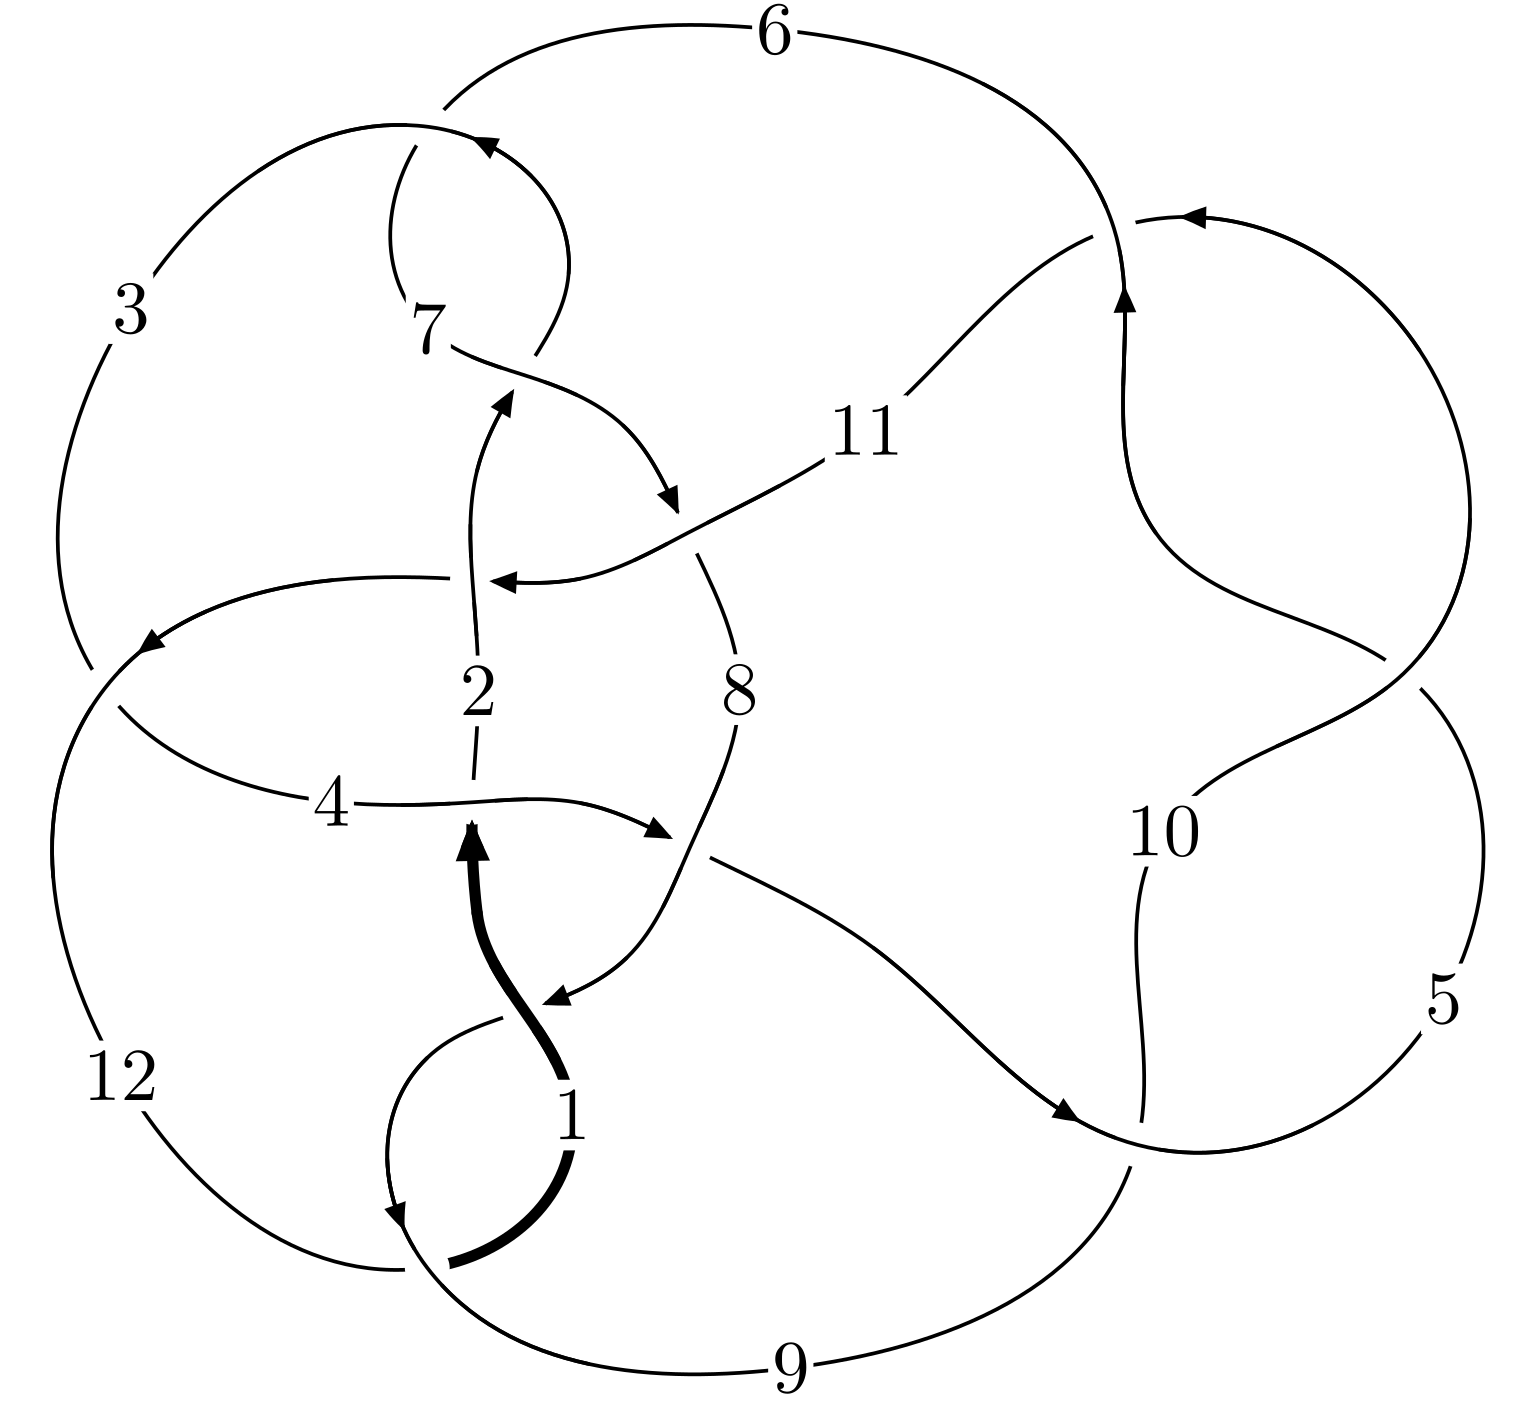
\includegraphics[width=112pt]{../../../GIT/diagram.site/Diagrams/png/1913_12a_1112.png}\\
\ \ \ A knot diagram\footnotemark}&
\allowdisplaybreaks
\textbf{Linearized knot diagam} \\
\cline{2-2}
 &
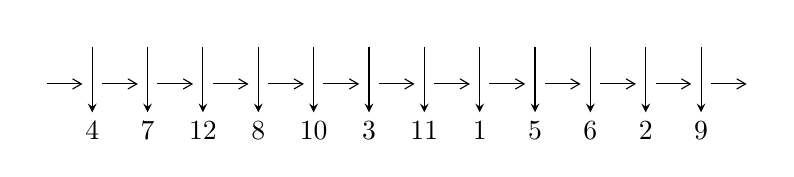
\begin{tikzpicture}[x=20pt, y=17pt]
	% nodes
	\node (C0) at (0, 0) {};
	\node (C1) at (1, 0) {};
	\node (C1U) at (1, +1) {};
	\node (C1D) at (1, -1) {4};

	\node (C2) at (2, 0) {};
	\node (C2U) at (2, +1) {};
	\node (C2D) at (2, -1) {7};

	\node (C3) at (3, 0) {};
	\node (C3U) at (3, +1) {};
	\node (C3D) at (3, -1) {12};

	\node (C4) at (4, 0) {};
	\node (C4U) at (4, +1) {};
	\node (C4D) at (4, -1) {8};

	\node (C5) at (5, 0) {};
	\node (C5U) at (5, +1) {};
	\node (C5D) at (5, -1) {10};

	\node (C6) at (6, 0) {};
	\node (C6U) at (6, +1) {};
	\node (C6D) at (6, -1) {3};

	\node (C7) at (7, 0) {};
	\node (C7U) at (7, +1) {};
	\node (C7D) at (7, -1) {11};

	\node (C8) at (8, 0) {};
	\node (C8U) at (8, +1) {};
	\node (C8D) at (8, -1) {1};

	\node (C9) at (9, 0) {};
	\node (C9U) at (9, +1) {};
	\node (C9D) at (9, -1) {5};

	\node (C10) at (10, 0) {};
	\node (C10U) at (10, +1) {};
	\node (C10D) at (10, -1) {6};

	\node (C11) at (11, 0) {};
	\node (C11U) at (11, +1) {};
	\node (C11D) at (11, -1) {2};

	\node (C12) at (12, 0) {};
	\node (C12U) at (12, +1) {};
	\node (C12D) at (12, -1) {9};
	\node (C13) at (13, 0) {};

	% arrows
	\draw[->,>={angle 60}]
	(C0) edge (C1) (C1) edge (C2) (C2) edge (C3) (C3) edge (C4) (C4) edge (C5) (C5) edge (C6) (C6) edge (C7) (C7) edge (C8) (C8) edge (C9) (C9) edge (C10) (C10) edge (C11) (C11) edge (C12) (C12) edge (C13) ;	\draw[->,>=stealth]
	(C1U) edge (C1D) (C2U) edge (C2D) (C3U) edge (C3D) (C4U) edge (C4D) (C5U) edge (C5D) (C6U) edge (C6D) (C7U) edge (C7D) (C8U) edge (C8D) (C9U) edge (C9D) (C10U) edge (C10D) (C11U) edge (C11D) (C12U) edge (C12D) ;
	\end{tikzpicture} \\
\hhline{~~} \\& 
\textbf{Solving Sequence} \\ \cline{2-2} 
 &
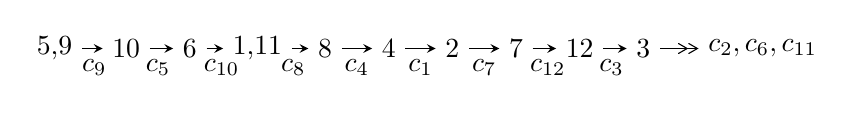
\begin{tikzpicture}[x=23pt, y=7pt]
	% node
	\node (A0) at (-1/8, 0) {5,9};
	\node (A1) at (1, 0) {10};
	\node (A2) at (2, 0) {6};
	\node (A3) at (49/16, 0) {1,11};
	\node (A4) at (33/8, 0) {8};
	\node (A5) at (41/8, 0) {4};
	\node (A6) at (49/8, 0) {2};
	\node (A7) at (57/8, 0) {7};
	\node (A8) at (65/8, 0) {12};
	\node (A9) at (73/8, 0) {3};
	\node (C1) at (1/2, -1) {$c_{9}$};
	\node (C2) at (3/2, -1) {$c_{5}$};
	\node (C3) at (5/2, -1) {$c_{10}$};
	\node (C4) at (29/8, -1) {$c_{8}$};
	\node (C5) at (37/8, -1) {$c_{4}$};
	\node (C6) at (45/8, -1) {$c_{1}$};
	\node (C7) at (53/8, -1) {$c_{7}$};
	\node (C8) at (61/8, -1) {$c_{12}$};
	\node (C9) at (69/8, -1) {$c_{3}$};
	\node (A10) at (11, 0) {$c_{2},c_{6},c_{11}$};

	% edge
	\draw[->,>=stealth]	
	(A0) edge (A1) (A1) edge (A2) (A2) edge (A3) (A3) edge (A4) (A4) edge (A5) (A5) edge (A6) (A6) edge (A7) (A7) edge (A8) (A8) edge (A9) ;
	\draw[->>,>={angle 60}]	
	(A9) edge (A10);
\end{tikzpicture} \\ 

\end{tabular} \\

\footnotetext{
The image of knot diagram is generated by the software ``\textbf{Draw programme}" developed by Andrew Bartholomew(\url{http://www.layer8.co.uk/maths/draw/index.htm\#Running-draw}), where we modified some parts for our purpose(\url{https://github.com/CATsTAILs/LinksPainter}).
}\phantom \\ \newline 
\centering \textbf{Ideals for irreducible components\footnotemark of $X_{\text{par}}$} 
 
\begin{align*}
I^u_{1}&=\langle 
1.05333\times10^{25} u^{34}-9.66699\times10^{25} u^{33}+\cdots+3.46689\times10^{24} b-2.06621\times10^{26},\\
\phantom{I^u_{1}}&\phantom{= \langle  }1.39674\times10^{26} u^{34}-1.16817\times10^{27} u^{33}+\cdots+1.73345\times10^{25} a-1.66150\times10^{27},\\
\phantom{I^u_{1}}&\phantom{= \langle  }u^{35}-10 u^{34}+\cdots+34 u+20\rangle \\
I^u_{2}&=\langle 
-4.36663\times10^{46} a u^{54}+3.92439\times10^{46} u^{54}+\cdots+1.93672\times10^{46} a-3.95313\times10^{46},\\
\phantom{I^u_{2}}&\phantom{= \langle  }-5.04902\times10^{42} a u^{54}+3.03401\times10^{43} u^{54}+\cdots-1.84231\times10^{44} a+2.06530\times10^{44},\\
\phantom{I^u_{2}}&\phantom{= \langle  }u^{55}+4 u^{54}+\cdots+3 u-1\rangle \\
I^u_{3}&=\langle 
- u^7+5 u^5-7 u^3+2 u^2+b-1,\;u^7-5 u^5+7 u^3-2 u^2+a+2,\;u^8- u^7-5 u^6+5 u^5+7 u^4-8 u^3+2 u^2- u-1\rangle \\
I^u_{4}&=\langle 
5 u^{14} a- u^{14}+\cdots- a-6,\;- u^{14} a- u^{13} a+\cdots+5 a+1,\\
\phantom{I^u_{4}}&\phantom{= \langle  }u^{15}+u^{14}-9 u^{13}-10 u^{12}+29 u^{11}+35 u^{10}-39 u^9-50 u^8+18 u^7+20 u^6-2 u^5+11 u^4+4 u^3-7 u^2-2 u-1\rangle \\
\\
\end{align*}
\raggedright * 4 irreducible components of $\dim_{\mathbb{C}}=0$, with total 183 representations.\\
\footnotetext{All coefficients of polynomials are rational numbers. But the coefficients are sometimes approximated in decimal forms when there is not enough margin.}
\newpage
\renewcommand{\arraystretch}{1}
\centering \section*{I. $I^u_{1}= \langle 1.05\times10^{25} u^{34}-9.67\times10^{25} u^{33}+\cdots+3.47\times10^{24} b-2.07\times10^{26},\;1.40\times10^{26} u^{34}-1.17\times10^{27} u^{33}+\cdots+1.73\times10^{25} a-1.66\times10^{27},\;u^{35}-10 u^{34}+\cdots+34 u+20 \rangle$}
\flushleft \textbf{(i) Arc colorings}\\
\begin{tabular}{m{7pt} m{180pt} m{7pt} m{180pt} }
\flushright $a_{5}=$&$\begin{pmatrix}0\\u\end{pmatrix}$ \\
\flushright $a_{9}=$&$\begin{pmatrix}1\\0\end{pmatrix}$ \\
\flushright $a_{10}=$&$\begin{pmatrix}1\\u^2\end{pmatrix}$ \\
\flushright $a_{6}=$&$\begin{pmatrix}- u\\- u^3+u\end{pmatrix}$ \\
\flushright $a_{1}=$&$\begin{pmatrix}-8.05760 u^{34}+67.3902 u^{33}+\cdots+216.775 u+95.8498\\-3.03824 u^{34}+27.8837 u^{33}+\cdots+151.183 u+59.5982\end{pmatrix}$ \\
\flushright $a_{11}=$&$\begin{pmatrix}- u^2+1\\- u^4+2 u^2\end{pmatrix}$ \\
\flushright $a_{8}=$&$\begin{pmatrix}-8.07945 u^{34}+70.9964 u^{33}+\cdots+308.907 u+126.677\\20.2058 u^{34}-172.098 u^{33}+\cdots-634.931 u-269.346\end{pmatrix}$ \\
\flushright $a_{4}=$&$\begin{pmatrix}0.743800 u^{34}-8.22710 u^{33}+\cdots-77.9988 u-27.7846\\-14.1624 u^{34}+122.356 u^{33}+\cdots+493.828 u+204.174\end{pmatrix}$ \\
\flushright $a_{2}=$&$\begin{pmatrix}-1.67496 u^{34}+12.9651 u^{33}+\cdots+17.1386 u+11.5788\\-4.24049 u^{34}+36.4664 u^{33}+\cdots+138.050 u+59.1818\end{pmatrix}$ \\
\flushright $a_{7}=$&$\begin{pmatrix}-6.69454 u^{34}+54.3723 u^{33}+\cdots+135.594 u+65.4843\\-2.18204 u^{34}+16.4361 u^{33}+\cdots+6.41141 u+8.93501\end{pmatrix}$ \\
\flushright $a_{12}=$&$\begin{pmatrix}-11.0958 u^{34}+95.2739 u^{33}+\cdots+367.957 u+155.448\\-3.03824 u^{34}+27.8837 u^{33}+\cdots+151.183 u+59.5982\end{pmatrix}$ \\
\flushright $a_{3}=$&$\begin{pmatrix}12.7046 u^{34}-108.535 u^{33}+\cdots-404.102 u-172.051\\10.5406 u^{34}-90.7723 u^{33}+\cdots-350.757 u-148.302\end{pmatrix}$\\&\end{tabular}
\flushleft \textbf{(ii) Obstruction class $= -1$}\\~\\
\flushleft \textbf{(iii) Cusp Shapes $= \frac{150582076995001786883398728}{1733446477044451037240759} u^{34}-\frac{1293993719851736952781608217}{1733446477044451037240759} u^{33}+\cdots-\frac{5021810385311596138829713842}{1733446477044451037240759} u-\frac{2132009033300635690695804090}{1733446477044451037240759}$}\\~\\
\newpage\renewcommand{\arraystretch}{1}
\flushleft \textbf{(iv) u-Polynomials at the component}\newline \\
\begin{tabular}{m{50pt}|m{274pt}}
Crossings & \hspace{64pt}u-Polynomials at each crossing \\
\hline $$\begin{aligned}c_{1},c_{11}\end{aligned}$$&$\begin{aligned}
&u^{35}+u^{34}+\cdots+7 u+1
\end{aligned}$\\
\hline $$\begin{aligned}c_{2},c_{6},c_{8}\\c_{12}\end{aligned}$$&$\begin{aligned}
&u^{35}+u^{34}+\cdots+8 u+4
\end{aligned}$\\
\hline $$\begin{aligned}c_{3}\end{aligned}$$&$\begin{aligned}
&u^{35}+19 u^{34}+\cdots+3582 u+412
\end{aligned}$\\
\hline $$\begin{aligned}c_{4},c_{7}\end{aligned}$$&$\begin{aligned}
&u^{35}+u^{34}+\cdots+4 u+1
\end{aligned}$\\
\hline $$\begin{aligned}c_{5},c_{9},c_{10}\end{aligned}$$&$\begin{aligned}
&u^{35}-10 u^{34}+\cdots+34 u+20
\end{aligned}$\\
\hline
\end{tabular}\\~\\
\newpage\renewcommand{\arraystretch}{1}
\flushleft \textbf{(v) Riley Polynomials at the component}\newline \\
\begin{tabular}{m{50pt}|m{274pt}}
Crossings & \hspace{64pt}Riley Polynomials at each crossing \\
\hline $$\begin{aligned}c_{1},c_{11}\end{aligned}$$&$\begin{aligned}
&y^{35}+25 y^{34}+\cdots+29 y-1
\end{aligned}$\\
\hline $$\begin{aligned}c_{2},c_{6},c_{8}\\c_{12}\end{aligned}$$&$\begin{aligned}
&y^{35}+23 y^{34}+\cdots+144 y-16
\end{aligned}$\\
\hline $$\begin{aligned}c_{3}\end{aligned}$$&$\begin{aligned}
&y^{35}+5 y^{34}+\cdots+3024300 y-169744
\end{aligned}$\\
\hline $$\begin{aligned}c_{4},c_{7}\end{aligned}$$&$\begin{aligned}
&y^{35}+11 y^{34}+\cdots-38 y-1
\end{aligned}$\\
\hline $$\begin{aligned}c_{5},c_{9},c_{10}\end{aligned}$$&$\begin{aligned}
&y^{35}-38 y^{34}+\cdots+1916 y-400
\end{aligned}$\\
\hline
\end{tabular}\\~\\
\newpage\flushleft \textbf{(vi) Complex Volumes and Cusp Shapes}
$$\begin{array}{c|c|c}  
\text{Solutions to }I^u_{1}& \I (\text{vol} + \sqrt{-1}CS) & \text{Cusp shape}\\
 \hline 
\begin{aligned}
u &= -0.803997 + 0.533074 I \\
a &= \phantom{-}1.43448 + 1.10830 I \\
b &= -0.062543 - 1.074790 I\end{aligned}
 & \phantom{-}6.06587 - 1.03841 I & -4.61661 + 0. I\phantom{ +0.000000I} \\ \hline\begin{aligned}
u &= -0.803997 - 0.533074 I \\
a &= \phantom{-}1.43448 - 1.10830 I \\
b &= -0.062543 + 1.074790 I\end{aligned}
 & \phantom{-}6.06587 + 1.03841 I & -4.61661 + 0. I\phantom{ +0.000000I} \\ \hline\begin{aligned}
u &= \phantom{-}1.105460 + 0.091312 I \\
a &= \phantom{-}0.064040 + 0.792479 I \\
b &= \phantom{-}0.422290 - 1.286260 I\end{aligned}
 & \phantom{-}3.42980 + 2.02749 I & -9.51115 + 1.18447 I \\ \hline\begin{aligned}
u &= \phantom{-}1.105460 - 0.091312 I \\
a &= \phantom{-}0.064040 - 0.792479 I \\
b &= \phantom{-}0.422290 + 1.286260 I\end{aligned}
 & \phantom{-}3.42980 - 2.02749 I & -9.51115 - 1.18447 I \\ \hline\begin{aligned}
u &= \phantom{-}0.673394 + 0.561518 I \\
a &= \phantom{-}0.676471 - 1.054270 I \\
b &= \phantom{-}0.207754 + 1.028490 I\end{aligned}
 & \phantom{-}2.46897 - 2.30248 I & -9.34144 + 3.82773 I \\ \hline\begin{aligned}
u &= \phantom{-}0.673394 - 0.561518 I \\
a &= \phantom{-}0.676471 + 1.054270 I \\
b &= \phantom{-}0.207754 - 1.028490 I\end{aligned}
 & \phantom{-}2.46897 + 2.30248 I & -9.34144 - 3.82773 I \\ \hline\begin{aligned}
u &= -0.598181 + 0.961731 I \\
a &= -0.54099 - 1.61027 I \\
b &= -0.538203 + 1.269780 I\end{aligned}
 & \phantom{-}6.0194 + 14.5123 I & -8.16245 - 9.90720 I \\ \hline\begin{aligned}
u &= -0.598181 - 0.961731 I \\
a &= -0.54099 + 1.61027 I \\
b &= -0.538203 - 1.269780 I\end{aligned}
 & \phantom{-}6.0194 - 14.5123 I & -8.16245 + 9.90720 I \\ \hline\begin{aligned}
u &= -0.473448 + 0.563117 I \\
a &= \phantom{-}0.348604 - 0.219293 I \\
b &= -0.867609 - 0.203863 I\end{aligned}
 & -0.63258 + 3.95481 I & -13.6290 - 6.0007 I \\ \hline\begin{aligned}
u &= -0.473448 - 0.563117 I \\
a &= \phantom{-}0.348604 + 0.219293 I \\
b &= -0.867609 + 0.203863 I\end{aligned}
 & -0.63258 - 3.95481 I & -13.6290 + 6.0007 I\\
 \hline 
 \end{array}$$\newpage$$\begin{array}{c|c|c}  
\text{Solutions to }I^u_{1}& \I (\text{vol} + \sqrt{-1}CS) & \text{Cusp shape}\\
 \hline 
\begin{aligned}
u &= -0.349085 + 0.606361 I \\
a &= \phantom{-}0.23813 + 2.73509 I \\
b &= \phantom{-}0.224450 - 1.246080 I\end{aligned}
 & \phantom{-}7.37225 + 4.97861 I & -1.44832 - 6.36788 I \\ \hline\begin{aligned}
u &= -0.349085 - 0.606361 I \\
a &= \phantom{-}0.23813 - 2.73509 I \\
b &= \phantom{-}0.224450 + 1.246080 I\end{aligned}
 & \phantom{-}7.37225 - 4.97861 I & -1.44832 + 6.36788 I \\ \hline\begin{aligned}
u &= -0.707100 + 1.117540 I \\
a &= -0.338530 - 1.076450 I \\
b &= \phantom{-}0.378752 + 1.180320 I\end{aligned}
 & \phantom{-}5.90335 - 7.84555 I & \phantom{-0.000000 } 0 \\ \hline\begin{aligned}
u &= -0.707100 - 1.117540 I \\
a &= -0.338530 + 1.076450 I \\
b &= \phantom{-}0.378752 - 1.180320 I\end{aligned}
 & \phantom{-}5.90335 + 7.84555 I & \phantom{-0.000000 } 0 \\ \hline\begin{aligned}
u &= -1.41227 + 0.14588 I \\
a &= \phantom{-}1.208100 + 0.092079 I \\
b &= \phantom{-}0.797088 - 0.998953 I\end{aligned}
 & \phantom{-}1.00471 + 6.09485 I & \phantom{-0.000000 } 0 \\ \hline\begin{aligned}
u &= -1.41227 - 0.14588 I \\
a &= \phantom{-}1.208100 - 0.092079 I \\
b &= \phantom{-}0.797088 + 0.998953 I\end{aligned}
 & \phantom{-}1.00471 - 6.09485 I & \phantom{-0.000000 } 0 \\ \hline\begin{aligned}
u &= -0.391148 + 0.427059 I \\
a &= \phantom{-}0.295079 + 0.998933 I \\
b &= \phantom{-}0.596218 - 0.096324 I\end{aligned}
 & -0.501599 - 0.453196 I & -14.2379 - 0.6217 I \\ \hline\begin{aligned}
u &= -0.391148 - 0.427059 I \\
a &= \phantom{-}0.295079 - 0.998933 I \\
b &= \phantom{-}0.596218 + 0.096324 I\end{aligned}
 & -0.501599 + 0.453196 I & -14.2379 + 0.6217 I \\ \hline\begin{aligned}
u &= \phantom{-}1.47231 + 0.17993 I \\
a &= -0.87718 + 1.36651 I \\
b &= -0.314810 - 1.360770 I\end{aligned}
 & \phantom{-}1.40292 - 7.73465 I & \phantom{-0.000000 } 0 \\ \hline\begin{aligned}
u &= \phantom{-}1.47231 - 0.17993 I \\
a &= -0.87718 - 1.36651 I \\
b &= -0.314810 + 1.360770 I\end{aligned}
 & \phantom{-}1.40292 + 7.73465 I & \phantom{-0.000000 } 0\\
 \hline 
 \end{array}$$\newpage$$\begin{array}{c|c|c}  
\text{Solutions to }I^u_{1}& \I (\text{vol} + \sqrt{-1}CS) & \text{Cusp shape}\\
 \hline 
\begin{aligned}
u &= \phantom{-}1.49385 + 0.19132 I \\
a &= \phantom{-}0.337606 - 0.343758 I \\
b &= \phantom{-}1.058070 - 0.319858 I\end{aligned}
 & -7.06787 - 6.71422 I & \phantom{-0.000000 } 0 \\ \hline\begin{aligned}
u &= \phantom{-}1.49385 - 0.19132 I \\
a &= \phantom{-}0.337606 + 0.343758 I \\
b &= \phantom{-}1.058070 + 0.319858 I\end{aligned}
 & -7.06787 + 6.71422 I & \phantom{-0.000000 } 0 \\ \hline\begin{aligned}
u &= \phantom{-}0.174543 + 0.422754 I \\
a &= -1.74538 + 2.01944 I \\
b &= -0.584132 - 1.136250 I\end{aligned}
 & \phantom{-}6.24160 - 4.06118 I & -1.88533 + 4.69388 I \\ \hline\begin{aligned}
u &= \phantom{-}0.174543 - 0.422754 I \\
a &= -1.74538 - 2.01944 I \\
b &= -0.584132 + 1.136250 I\end{aligned}
 & \phantom{-}6.24160 + 4.06118 I & -1.88533 - 4.69388 I \\ \hline\begin{aligned}
u &= -1.54135 + 0.10386 I \\
a &= -0.828626 - 0.343315 I \\
b &= -0.521454 + 0.940783 I\end{aligned}
 & -4.84166 + 4.34625 I & \phantom{-0.000000 } 0 \\ \hline\begin{aligned}
u &= -1.54135 - 0.10386 I \\
a &= -0.828626 + 0.343315 I \\
b &= -0.521454 - 0.940783 I\end{aligned}
 & -4.84166 - 4.34625 I & \phantom{-0.000000 } 0 \\ \hline\begin{aligned}
u &= \phantom{-}1.54823 + 0.03994 I \\
a &= -0.491121 + 0.284574 I \\
b &= -0.604028 + 0.080486 I\end{aligned}
 & -7.11890 - 0.61994 I & \phantom{-0.000000 } 0 \\ \hline\begin{aligned}
u &= \phantom{-}1.54823 - 0.03994 I \\
a &= -0.491121 - 0.284574 I \\
b &= -0.604028 - 0.080486 I\end{aligned}
 & -7.11890 + 0.61994 I & \phantom{-0.000000 } 0 \\ \hline\begin{aligned}
u &= \phantom{-}1.57837 + 0.33899 I \\
a &= \phantom{-}1.038850 - 0.942216 I \\
b &= \phantom{-}0.66578 + 1.28800 I\end{aligned}
 & -1.0151 - 19.2744 I & \phantom{-0.000000 } 0 \\ \hline\begin{aligned}
u &= \phantom{-}1.57837 - 0.33899 I \\
a &= \phantom{-}1.038850 + 0.942216 I \\
b &= \phantom{-}0.66578 - 1.28800 I\end{aligned}
 & -1.0151 + 19.2744 I & \phantom{-0.000000 } 0\\
 \hline 
 \end{array}$$\newpage$$\begin{array}{c|c|c}  
\text{Solutions to }I^u_{1}& \I (\text{vol} + \sqrt{-1}CS) & \text{Cusp shape}\\
 \hline 
\begin{aligned}
u &= -0.382332\phantom{ +0.000000I} \\
a &= \phantom{-}0.622554\phantom{ +0.000000I} \\
b &= \phantom{-}0.322801\phantom{ +0.000000I}\end{aligned}
 & -0.581792\phantom{ +0.000000I} & -17.0880\phantom{ +0.000000I} \\ \hline\begin{aligned}
u &= \phantom{-}1.53143 + 0.55845 I \\
a &= -0.701270 + 1.154460 I \\
b &= -0.300993 - 0.837192 I\end{aligned}
 & -3.88596 - 3.19348 I & \phantom{-0.000000 } 0 \\ \hline\begin{aligned}
u &= \phantom{-}1.53143 - 0.55845 I \\
a &= -0.701270 - 1.154460 I \\
b &= -0.300993 + 0.837192 I\end{aligned}
 & -3.88596 + 3.19348 I & \phantom{-0.000000 } 0 \\ \hline\begin{aligned}
u &= \phantom{-}1.89015 + 0.03404 I \\
a &= -0.329520 - 0.418059 I \\
b &= -0.218032 + 0.900975 I\end{aligned}
 & -3.86222 + 1.75896 I & \phantom{-0.000000 } 0 \\ \hline\begin{aligned}
u &= \phantom{-}1.89015 - 0.03404 I \\
a &= -0.329520 + 0.418059 I \\
b &= -0.218032 - 0.900975 I\end{aligned}
 & -3.86222 - 1.75896 I & \phantom{-0.000000 } 0\\
 \hline 
 \end{array}$$\newpage\newpage\renewcommand{\arraystretch}{1}
\centering \section*{II. $I^u_{2}= \langle -4.37\times10^{46} a u^{54}+3.92\times10^{46} u^{54}+\cdots+1.94\times10^{46} a-3.95\times10^{46},\;-5.05\times10^{42} a u^{54}+3.03\times10^{43} u^{54}+\cdots-1.84\times10^{44} a+2.07\times10^{44},\;u^{55}+4 u^{54}+\cdots+3 u-1 \rangle$}
\flushleft \textbf{(i) Arc colorings}\\
\begin{tabular}{m{7pt} m{180pt} m{7pt} m{180pt} }
\flushright $a_{5}=$&$\begin{pmatrix}0\\u\end{pmatrix}$ \\
\flushright $a_{9}=$&$\begin{pmatrix}1\\0\end{pmatrix}$ \\
\flushright $a_{10}=$&$\begin{pmatrix}1\\u^2\end{pmatrix}$ \\
\flushright $a_{6}=$&$\begin{pmatrix}- u\\- u^3+u\end{pmatrix}$ \\
\flushright $a_{1}=$&$\begin{pmatrix}a\\1.14957 a u^{54}-1.03314 u^{54}+\cdots-0.509865 a+1.04071\end{pmatrix}$ \\
\flushright $a_{11}=$&$\begin{pmatrix}- u^2+1\\- u^4+2 u^2\end{pmatrix}$ \\
\flushright $a_{8}=$&$\begin{pmatrix}-1.26663 a u^{54}-0.830110 u^{54}+\cdots+1.05263 a-3.29375\\-0.604358 a u^{54}+1.38963 u^{54}+\cdots-1.89616 a+2.18358\end{pmatrix}$ \\
\flushright $a_{4}=$&$\begin{pmatrix}0.459243 a u^{54}-2.31570 u^{54}+\cdots+1.32353 a-7.18383\\0.491567 a u^{54}+0.506314 u^{54}+\cdots-0.166689 a+0.246017\end{pmatrix}$ \\
\flushright $a_{2}=$&$\begin{pmatrix}-1.18307 a u^{54}+4.62717 u^{54}+\cdots-3.90624 a+6.59236\\-0.247329 a u^{54}-0.152341 u^{54}+\cdots-0.316387 a-1.04384\end{pmatrix}$ \\
\flushright $a_{7}=$&$\begin{pmatrix}-1.94504 a u^{54}+0.689214 u^{54}+\cdots-1.16001 a-0.436189\\-0.235673 a u^{54}+1.03979 u^{54}+\cdots-1.66571 a+2.18129\end{pmatrix}$ \\
\flushright $a_{12}=$&$\begin{pmatrix}1.14957 a u^{54}-1.03314 u^{54}+\cdots+0.490135 a+1.04071\\1.14957 a u^{54}-1.03314 u^{54}+\cdots-0.509865 a+1.04071\end{pmatrix}$ \\
\flushright $a_{3}=$&$\begin{pmatrix}0.468039 a u^{54}-2.67095 u^{54}+\cdots+1.96864 a-5.26709\\-0.0813838 a u^{54}+0.151068 u^{54}+\cdots+0.379373 a+2.16276\end{pmatrix}$\\&\end{tabular}
\flushleft \textbf{(ii) Obstruction class $= -1$}\\~\\
\flushleft \textbf{(iii) Cusp Shapes $= 0.650219 u^{54}+3.90679 u^{53}+\cdots+33.7462 u-13.9094$}\\~\\
\newpage\renewcommand{\arraystretch}{1}
\flushleft \textbf{(iv) u-Polynomials at the component}\newline \\
\begin{tabular}{m{50pt}|m{274pt}}
Crossings & \hspace{64pt}u-Polynomials at each crossing \\
\hline $$\begin{aligned}c_{1},c_{11}\end{aligned}$$&$\begin{aligned}
&u^{110}-10 u^{109}+\cdots-62239 u+5573
\end{aligned}$\\
\hline $$\begin{aligned}c_{2},c_{6},c_{8}\\c_{12}\end{aligned}$$&$\begin{aligned}
&u^{110}- u^{109}+\cdots+757 u+161
\end{aligned}$\\
\hline $$\begin{aligned}c_{3}\end{aligned}$$&$\begin{aligned}
&(u^{55}-8 u^{54}+\cdots+u-1)^{2}
\end{aligned}$\\
\hline $$\begin{aligned}c_{4},c_{7}\end{aligned}$$&$\begin{aligned}
&u^{110}+5 u^{109}+\cdots-2143 u+1273
\end{aligned}$\\
\hline $$\begin{aligned}c_{5},c_{9},c_{10}\end{aligned}$$&$\begin{aligned}
&(u^{55}+4 u^{54}+\cdots+3 u-1)^{2}
\end{aligned}$\\
\hline
\end{tabular}\\~\\
\newpage\renewcommand{\arraystretch}{1}
\flushleft \textbf{(v) Riley Polynomials at the component}\newline \\
\begin{tabular}{m{50pt}|m{274pt}}
Crossings & \hspace{64pt}Riley Polynomials at each crossing \\
\hline $$\begin{aligned}c_{1},c_{11}\end{aligned}$$&$\begin{aligned}
&y^{110}+18 y^{109}+\cdots+573371397 y+31058329
\end{aligned}$\\
\hline $$\begin{aligned}c_{2},c_{6},c_{8}\\c_{12}\end{aligned}$$&$\begin{aligned}
&y^{110}+53 y^{109}+\cdots+1093301 y+25921
\end{aligned}$\\
\hline $$\begin{aligned}c_{3}\end{aligned}$$&$\begin{aligned}
&(y^{55}+52 y^{53}+\cdots-51 y-1)^{2}
\end{aligned}$\\
\hline $$\begin{aligned}c_{4},c_{7}\end{aligned}$$&$\begin{aligned}
&y^{110}-19 y^{109}+\cdots+173836323 y+1620529
\end{aligned}$\\
\hline $$\begin{aligned}c_{5},c_{9},c_{10}\end{aligned}$$&$\begin{aligned}
&(y^{55}-58 y^{54}+\cdots+y-1)^{2}
\end{aligned}$\\
\hline
\end{tabular}\\~\\
\newpage\flushleft \textbf{(vi) Complex Volumes and Cusp Shapes}
$$\begin{array}{c|c|c}  
\text{Solutions to }I^u_{2}& \I (\text{vol} + \sqrt{-1}CS) & \text{Cusp shape}\\
 \hline 
\begin{aligned}
u &= \phantom{-}0.690905 + 0.836192 I \\
a &= \phantom{-}0.366866 - 0.880523 I \\
b &= -0.241428 + 0.824984 I\end{aligned}
 & \phantom{-}2.29186 - 2.97653 I & \phantom{-0.000000 } 0 \\ \hline\begin{aligned}
u &= \phantom{-}0.690905 + 0.836192 I \\
a &= \phantom{-}0.61526 - 1.37416 I \\
b &= \phantom{-}0.455751 + 1.178700 I\end{aligned}
 & \phantom{-}2.29186 - 2.97653 I & \phantom{-0.000000 } 0 \\ \hline\begin{aligned}
u &= \phantom{-}0.690905 - 0.836192 I \\
a &= \phantom{-}0.366866 + 0.880523 I \\
b &= -0.241428 - 0.824984 I\end{aligned}
 & \phantom{-}2.29186 + 2.97653 I & \phantom{-0.000000 } 0 \\ \hline\begin{aligned}
u &= \phantom{-}0.690905 - 0.836192 I \\
a &= \phantom{-}0.61526 + 1.37416 I \\
b &= \phantom{-}0.455751 - 1.178700 I\end{aligned}
 & \phantom{-}2.29186 + 2.97653 I & \phantom{-0.000000 } 0 \\ \hline\begin{aligned}
u &= -0.211935 + 1.078880 I \\
a &= \phantom{-}0.14003 + 1.43194 I \\
b &= \phantom{-}0.470912 - 1.207600 I\end{aligned}
 & \phantom{-}2.01266 + 5.69803 I & \phantom{-0.000000 } 0 \\ \hline\begin{aligned}
u &= -0.211935 + 1.078880 I \\
a &= -0.05804 - 1.67565 I \\
b &= -0.253274 + 0.756122 I\end{aligned}
 & \phantom{-}2.01266 + 5.69803 I & \phantom{-0.000000 } 0 \\ \hline\begin{aligned}
u &= -0.211935 - 1.078880 I \\
a &= \phantom{-}0.14003 - 1.43194 I \\
b &= \phantom{-}0.470912 + 1.207600 I\end{aligned}
 & \phantom{-}2.01266 - 5.69803 I & \phantom{-0.000000 } 0 \\ \hline\begin{aligned}
u &= -0.211935 - 1.078880 I \\
a &= -0.05804 + 1.67565 I \\
b &= -0.253274 - 0.756122 I\end{aligned}
 & \phantom{-}2.01266 - 5.69803 I & \phantom{-0.000000 } 0 \\ \hline\begin{aligned}
u &= \phantom{-}0.490640 + 0.738991 I \\
a &= \phantom{-}0.160306 + 0.008195 I \\
b &= -1.008690 + 0.095297 I\end{aligned}
 & \phantom{-}2.39208 - 9.05536 I & -10.63523 + 8.54922 I \\ \hline\begin{aligned}
u &= \phantom{-}0.490640 + 0.738991 I \\
a &= -0.74005 + 1.97245 I \\
b &= -0.532272 - 1.198920 I\end{aligned}
 & \phantom{-}2.39208 - 9.05536 I & -10.63523 + 8.54922 I\\
 \hline 
 \end{array}$$\newpage$$\begin{array}{c|c|c}  
\text{Solutions to }I^u_{2}& \I (\text{vol} + \sqrt{-1}CS) & \text{Cusp shape}\\
 \hline 
\begin{aligned}
u &= \phantom{-}0.490640 - 0.738991 I \\
a &= \phantom{-}0.160306 - 0.008195 I \\
b &= -1.008690 - 0.095297 I\end{aligned}
 & \phantom{-}2.39208 + 9.05536 I & -10.63523 - 8.54922 I \\ \hline\begin{aligned}
u &= \phantom{-}0.490640 - 0.738991 I \\
a &= -0.74005 - 1.97245 I \\
b &= -0.532272 + 1.198920 I\end{aligned}
 & \phantom{-}2.39208 + 9.05536 I & -10.63523 - 8.54922 I \\ \hline\begin{aligned}
u &= \phantom{-}0.721236 + 0.487051 I \\
a &= -0.175549 - 0.965280 I \\
b &= \phantom{-}0.265285 + 0.402133 I\end{aligned}
 & \phantom{-}2.64516 - 3.21436 I & -11.40156 + 4.88184 I \\ \hline\begin{aligned}
u &= \phantom{-}0.721236 + 0.487051 I \\
a &= \phantom{-}1.32499 - 1.39029 I \\
b &= \phantom{-}0.439519 + 1.129730 I\end{aligned}
 & \phantom{-}2.64516 - 3.21436 I & -11.40156 + 4.88184 I \\ \hline\begin{aligned}
u &= \phantom{-}0.721236 - 0.487051 I \\
a &= -0.175549 + 0.965280 I \\
b &= \phantom{-}0.265285 - 0.402133 I\end{aligned}
 & \phantom{-}2.64516 + 3.21436 I & -11.40156 - 4.88184 I \\ \hline\begin{aligned}
u &= \phantom{-}0.721236 - 0.487051 I \\
a &= \phantom{-}1.32499 + 1.39029 I \\
b &= \phantom{-}0.439519 - 1.129730 I\end{aligned}
 & \phantom{-}2.64516 + 3.21436 I & -11.40156 - 4.88184 I \\ \hline\begin{aligned}
u &= -0.094135 + 0.797521 I \\
a &= -0.09523 + 1.51095 I \\
b &= -0.33150 - 1.38137 I\end{aligned}
 & \phantom{-}7.37231 + 4.07544 I & -3.25549 - 3.99001 I \\ \hline\begin{aligned}
u &= -0.094135 + 0.797521 I \\
a &= \phantom{-}0.19906 - 2.27702 I \\
b &= -0.400816 + 1.176110 I\end{aligned}
 & \phantom{-}7.37231 + 4.07544 I & -3.25549 - 3.99001 I \\ \hline\begin{aligned}
u &= -0.094135 - 0.797521 I \\
a &= -0.09523 - 1.51095 I \\
b &= -0.33150 + 1.38137 I\end{aligned}
 & \phantom{-}7.37231 - 4.07544 I & -3.25549 + 3.99001 I \\ \hline\begin{aligned}
u &= -0.094135 - 0.797521 I \\
a &= \phantom{-}0.19906 + 2.27702 I \\
b &= -0.400816 - 1.176110 I\end{aligned}
 & \phantom{-}7.37231 - 4.07544 I & -3.25549 + 3.99001 I\\
 \hline 
 \end{array}$$\newpage$$\begin{array}{c|c|c}  
\text{Solutions to }I^u_{2}& \I (\text{vol} + \sqrt{-1}CS) & \text{Cusp shape}\\
 \hline 
\begin{aligned}
u &= -0.659238 + 0.334521 I \\
a &= \phantom{-}0.942611 + 0.016242 I \\
b &= -0.252937 - 0.954465 I\end{aligned}
 & -0.69659 - 1.57624 I & -16.2076 + 2.4005 I \\ \hline\begin{aligned}
u &= -0.659238 + 0.334521 I \\
a &= \phantom{-}0.097853 - 0.336057 I \\
b &= \phantom{-}0.839956 + 0.182273 I\end{aligned}
 & -0.69659 - 1.57624 I & -16.2076 + 2.4005 I \\ \hline\begin{aligned}
u &= -0.659238 - 0.334521 I \\
a &= \phantom{-}0.942611 - 0.016242 I \\
b &= -0.252937 + 0.954465 I\end{aligned}
 & -0.69659 + 1.57624 I & -16.2076 - 2.4005 I \\ \hline\begin{aligned}
u &= -0.659238 - 0.334521 I \\
a &= \phantom{-}0.097853 + 0.336057 I \\
b &= \phantom{-}0.839956 - 0.182273 I\end{aligned}
 & -0.69659 + 1.57624 I & -16.2076 - 2.4005 I \\ \hline\begin{aligned}
u &= -1.174720 + 0.534428 I \\
a &= -0.647509 - 0.837083 I \\
b &= \phantom{-}0.303605 + 1.014120 I\end{aligned}
 & \phantom{-}4.16724 + 0.68269 I & \phantom{-0.000000 } 0 \\ \hline\begin{aligned}
u &= -1.174720 + 0.534428 I \\
a &= \phantom{-}1.009840 + 0.600097 I \\
b &= \phantom{-}0.651657 - 1.213950 I\end{aligned}
 & \phantom{-}4.16724 + 0.68269 I & \phantom{-0.000000 } 0 \\ \hline\begin{aligned}
u &= -1.174720 - 0.534428 I \\
a &= -0.647509 + 0.837083 I \\
b &= \phantom{-}0.303605 - 1.014120 I\end{aligned}
 & \phantom{-}4.16724 - 0.68269 I & \phantom{-0.000000 } 0 \\ \hline\begin{aligned}
u &= -1.174720 - 0.534428 I \\
a &= \phantom{-}1.009840 - 0.600097 I \\
b &= \phantom{-}0.651657 + 1.213950 I\end{aligned}
 & \phantom{-}4.16724 - 0.68269 I & \phantom{-0.000000 } 0 \\ \hline\begin{aligned}
u &= \phantom{-}0.512258 + 0.483347 I \\
a &= -0.83422 + 1.25390 I \\
b &= \phantom{-}0.478814 - 1.088540 I\end{aligned}
 & \phantom{-}2.16174 + 4.57220 I & -12.69275 - 5.26611 I \\ \hline\begin{aligned}
u &= \phantom{-}0.512258 + 0.483347 I \\
a &= \phantom{-}1.01988 - 1.23393 I \\
b &= \phantom{-}0.518200 - 0.362883 I\end{aligned}
 & \phantom{-}2.16174 + 4.57220 I & -12.69275 - 5.26611 I\\
 \hline 
 \end{array}$$\newpage$$\begin{array}{c|c|c}  
\text{Solutions to }I^u_{2}& \I (\text{vol} + \sqrt{-1}CS) & \text{Cusp shape}\\
 \hline 
\begin{aligned}
u &= \phantom{-}0.512258 - 0.483347 I \\
a &= -0.83422 - 1.25390 I \\
b &= \phantom{-}0.478814 + 1.088540 I\end{aligned}
 & \phantom{-}2.16174 - 4.57220 I & -12.69275 + 5.26611 I \\ \hline\begin{aligned}
u &= \phantom{-}0.512258 - 0.483347 I \\
a &= \phantom{-}1.01988 + 1.23393 I \\
b &= \phantom{-}0.518200 + 0.362883 I\end{aligned}
 & \phantom{-}2.16174 - 4.57220 I & -12.69275 + 5.26611 I \\ \hline\begin{aligned}
u &= -1.305390 + 0.111278 I \\
a &= -0.162667 - 0.719844 I \\
b &= \phantom{-}0.085396 + 1.348090 I\end{aligned}
 & -0.64381 + 2.74769 I & \phantom{-0.000000 } 0 \\ \hline\begin{aligned}
u &= -1.305390 + 0.111278 I \\
a &= \phantom{-}0.158184 + 0.340349 I \\
b &= \phantom{-}0.890640 + 0.025319 I\end{aligned}
 & -0.64381 + 2.74769 I & \phantom{-0.000000 } 0 \\ \hline\begin{aligned}
u &= -1.305390 - 0.111278 I \\
a &= -0.162667 + 0.719844 I \\
b &= \phantom{-}0.085396 - 1.348090 I\end{aligned}
 & -0.64381 - 2.74769 I & \phantom{-0.000000 } 0 \\ \hline\begin{aligned}
u &= -1.305390 - 0.111278 I \\
a &= \phantom{-}0.158184 - 0.340349 I \\
b &= \phantom{-}0.890640 - 0.025319 I\end{aligned}
 & -0.64381 - 2.74769 I & \phantom{-0.000000 } 0 \\ \hline\begin{aligned}
u &= \phantom{-}1.321550 + 0.221317 I \\
a &= -0.130536 + 0.598890 I \\
b &= \phantom{-}0.04613 - 1.58841 I\end{aligned}
 & \phantom{-}3.02817 - 7.64203 I & \phantom{-0.000000 } 0 \\ \hline\begin{aligned}
u &= \phantom{-}1.321550 + 0.221317 I \\
a &= \phantom{-}1.17454 - 1.37975 I \\
b &= \phantom{-}0.486101 + 1.244880 I\end{aligned}
 & \phantom{-}3.02817 - 7.64203 I & \phantom{-0.000000 } 0 \\ \hline\begin{aligned}
u &= \phantom{-}1.321550 - 0.221317 I \\
a &= -0.130536 - 0.598890 I \\
b &= \phantom{-}0.04613 + 1.58841 I\end{aligned}
 & \phantom{-}3.02817 + 7.64203 I & \phantom{-0.000000 } 0 \\ \hline\begin{aligned}
u &= \phantom{-}1.321550 - 0.221317 I \\
a &= \phantom{-}1.17454 + 1.37975 I \\
b &= \phantom{-}0.486101 - 1.244880 I\end{aligned}
 & \phantom{-}3.02817 + 7.64203 I & \phantom{-0.000000 } 0\\
 \hline 
 \end{array}$$\newpage$$\begin{array}{c|c|c}  
\text{Solutions to }I^u_{2}& \I (\text{vol} + \sqrt{-1}CS) & \text{Cusp shape}\\
 \hline 
\begin{aligned}
u &= \phantom{-}1.34005\phantom{ +0.000000I} \\
a &= \phantom{-}1.353980 + 0.139540 I \\
b &= \phantom{-}0.760771 - 0.965542 I\end{aligned}
 & \phantom{-}0.940013\phantom{ +0.000000I} & \phantom{-0.000000 } 0 \\ \hline\begin{aligned}
u &= \phantom{-}1.34005\phantom{ +0.000000I} \\
a &= \phantom{-}1.353980 - 0.139540 I \\
b &= \phantom{-}0.760771 + 0.965542 I\end{aligned}
 & \phantom{-}0.940013\phantom{ +0.000000I} & \phantom{-0.000000 } 0 \\ \hline\begin{aligned}
u &= \phantom{-}1.34292\phantom{ +0.000000I} \\
a &= -1.22526 + 0.74618 I \\
b &= -0.485734 - 0.832040 I\end{aligned}
 & -4.96750\phantom{ +0.000000I} & \phantom{-0.000000 } 0 \\ \hline\begin{aligned}
u &= \phantom{-}1.34292\phantom{ +0.000000I} \\
a &= -1.22526 - 0.74618 I \\
b &= -0.485734 + 0.832040 I\end{aligned}
 & -4.96750\phantom{ +0.000000I} & \phantom{-0.000000 } 0 \\ \hline\begin{aligned}
u &= -1.386050 + 0.039559 I \\
a &= -0.470371 + 0.137165 I \\
b &= -1.43986 + 0.40976 I\end{aligned}
 & -5.51949 + 1.85437 I & \phantom{-0.000000 } 0 \\ \hline\begin{aligned}
u &= -1.386050 + 0.039559 I \\
a &= \phantom{-}1.53412 + 1.58546 I \\
b &= \phantom{-}0.370669 - 1.035590 I\end{aligned}
 & -5.51949 + 1.85437 I & \phantom{-0.000000 } 0 \\ \hline\begin{aligned}
u &= -1.386050 - 0.039559 I \\
a &= -0.470371 - 0.137165 I \\
b &= -1.43986 - 0.40976 I\end{aligned}
 & -5.51949 - 1.85437 I & \phantom{-0.000000 } 0 \\ \hline\begin{aligned}
u &= -1.386050 - 0.039559 I \\
a &= \phantom{-}1.53412 - 1.58546 I \\
b &= \phantom{-}0.370669 + 1.035590 I\end{aligned}
 & -5.51949 - 1.85437 I & \phantom{-0.000000 } 0 \\ \hline\begin{aligned}
u &= \phantom{-}1.387900 + 0.064924 I \\
a &= -0.983235 + 0.686959 I \\
b &= -0.77404 - 1.32545 I\end{aligned}
 & -2.42366 - 5.71620 I & \phantom{-0.000000 } 0 \\ \hline\begin{aligned}
u &= \phantom{-}1.387900 + 0.064924 I \\
a &= \phantom{-}1.68695 + 1.28000 I \\
b &= \phantom{-}0.303534 - 0.933624 I\end{aligned}
 & -2.42366 - 5.71620 I & \phantom{-0.000000 } 0\\
 \hline 
 \end{array}$$\newpage$$\begin{array}{c|c|c}  
\text{Solutions to }I^u_{2}& \I (\text{vol} + \sqrt{-1}CS) & \text{Cusp shape}\\
 \hline 
\begin{aligned}
u &= \phantom{-}1.387900 - 0.064924 I \\
a &= -0.983235 - 0.686959 I \\
b &= -0.77404 + 1.32545 I\end{aligned}
 & -2.42366 + 5.71620 I & \phantom{-0.000000 } 0 \\ \hline\begin{aligned}
u &= \phantom{-}1.387900 - 0.064924 I \\
a &= \phantom{-}1.68695 - 1.28000 I \\
b &= \phantom{-}0.303534 + 0.933624 I\end{aligned}
 & -2.42366 + 5.71620 I & \phantom{-0.000000 } 0 \\ \hline\begin{aligned}
u &= \phantom{-}0.225296 + 0.549556 I \\
a &= \phantom{-}0.905062 - 0.259449 I \\
b &= -0.570153 - 0.065197 I\end{aligned}
 & \phantom{-}3.94023 - 0.36163 I & -6.60083 + 2.19067 I \\ \hline\begin{aligned}
u &= \phantom{-}0.225296 + 0.549556 I \\
a &= \phantom{-}0.42046 - 2.13735 I \\
b &= -0.288357 + 1.170460 I\end{aligned}
 & \phantom{-}3.94023 - 0.36163 I & -6.60083 + 2.19067 I \\ \hline\begin{aligned}
u &= \phantom{-}0.225296 - 0.549556 I \\
a &= \phantom{-}0.905062 + 0.259449 I \\
b &= -0.570153 + 0.065197 I\end{aligned}
 & \phantom{-}3.94023 + 0.36163 I & -6.60083 - 2.19067 I \\ \hline\begin{aligned}
u &= \phantom{-}0.225296 - 0.549556 I \\
a &= \phantom{-}0.42046 + 2.13735 I \\
b &= -0.288357 - 1.170460 I\end{aligned}
 & \phantom{-}3.94023 + 0.36163 I & -6.60083 - 2.19067 I \\ \hline\begin{aligned}
u &= -1.386690 + 0.269417 I \\
a &= -0.422386 - 0.146904 I \\
b &= -1.216850 - 0.506933 I\end{aligned}
 & -6.24126 + 4.08987 I & \phantom{-0.000000 } 0 \\ \hline\begin{aligned}
u &= -1.386690 + 0.269417 I \\
a &= \phantom{-}0.69726 + 1.42412 I \\
b &= \phantom{-}0.456342 - 0.987921 I\end{aligned}
 & -6.24126 + 4.08987 I & \phantom{-0.000000 } 0 \\ \hline\begin{aligned}
u &= -1.386690 - 0.269417 I \\
a &= -0.422386 + 0.146904 I \\
b &= -1.216850 + 0.506933 I\end{aligned}
 & -6.24126 - 4.08987 I & \phantom{-0.000000 } 0 \\ \hline\begin{aligned}
u &= -1.386690 - 0.269417 I \\
a &= \phantom{-}0.69726 - 1.42412 I \\
b &= \phantom{-}0.456342 + 0.987921 I\end{aligned}
 & -6.24126 - 4.08987 I & \phantom{-0.000000 } 0\\
 \hline 
 \end{array}$$\newpage$$\begin{array}{c|c|c}  
\text{Solutions to }I^u_{2}& \I (\text{vol} + \sqrt{-1}CS) & \text{Cusp shape}\\
 \hline 
\begin{aligned}
u &= \phantom{-}0.536397 + 0.236810 I \\
a &= -1.26961 - 1.53747 I \\
b &= -0.213339 - 1.096540 I\end{aligned}
 & \phantom{-}4.05157 - 6.54678 I & -9.8538 + 10.2390 I \\ \hline\begin{aligned}
u &= \phantom{-}0.536397 + 0.236810 I \\
a &= \phantom{-}1.08706 - 1.94734 I \\
b &= \phantom{-}0.49841 + 1.34996 I\end{aligned}
 & \phantom{-}4.05157 - 6.54678 I & -9.8538 + 10.2390 I \\ \hline\begin{aligned}
u &= \phantom{-}0.536397 - 0.236810 I \\
a &= -1.26961 + 1.53747 I \\
b &= -0.213339 + 1.096540 I\end{aligned}
 & \phantom{-}4.05157 + 6.54678 I & -9.8538 - 10.2390 I \\ \hline\begin{aligned}
u &= \phantom{-}0.536397 - 0.236810 I \\
a &= \phantom{-}1.08706 + 1.94734 I \\
b &= \phantom{-}0.49841 - 1.34996 I\end{aligned}
 & \phantom{-}4.05157 + 6.54678 I & -9.8538 - 10.2390 I \\ \hline\begin{aligned}
u &= \phantom{-}0.126349 + 0.501505 I \\
a &= \phantom{-}0.133217 + 0.639727 I \\
b &= \phantom{-}0.878362 - 0.065344 I\end{aligned}
 & -1.43716 - 0.99063 I & -13.8892 + 7.3873 I \\ \hline\begin{aligned}
u &= \phantom{-}0.126349 + 0.501505 I \\
a &= \phantom{-}0.54521 + 2.88272 I \\
b &= -0.256700 - 0.705954 I\end{aligned}
 & -1.43716 - 0.99063 I & -13.8892 + 7.3873 I \\ \hline\begin{aligned}
u &= \phantom{-}0.126349 - 0.501505 I \\
a &= \phantom{-}0.133217 - 0.639727 I \\
b &= \phantom{-}0.878362 + 0.065344 I\end{aligned}
 & -1.43716 + 0.99063 I & -13.8892 - 7.3873 I \\ \hline\begin{aligned}
u &= \phantom{-}0.126349 - 0.501505 I \\
a &= \phantom{-}0.54521 - 2.88272 I \\
b &= -0.256700 + 0.705954 I\end{aligned}
 & -1.43716 + 0.99063 I & -13.8892 - 7.3873 I \\ \hline\begin{aligned}
u &= \phantom{-}1.52074 + 0.01580 I \\
a &= -0.266906 + 0.895049 I \\
b &= \phantom{-}0.111980 + 0.556616 I\end{aligned}
 & -7.32030 - 0.96544 I & \phantom{-0.000000 } 0 \\ \hline\begin{aligned}
u &= \phantom{-}1.52074 + 0.01580 I \\
a &= -0.443060 + 0.172960 I \\
b &= -1.240360 + 0.064281 I\end{aligned}
 & -7.32030 - 0.96544 I & \phantom{-0.000000 } 0\\
 \hline 
 \end{array}$$\newpage$$\begin{array}{c|c|c}  
\text{Solutions to }I^u_{2}& \I (\text{vol} + \sqrt{-1}CS) & \text{Cusp shape}\\
 \hline 
\begin{aligned}
u &= \phantom{-}1.52074 - 0.01580 I \\
a &= -0.266906 - 0.895049 I \\
b &= \phantom{-}0.111980 - 0.556616 I\end{aligned}
 & -7.32030 + 0.96544 I & \phantom{-0.000000 } 0 \\ \hline\begin{aligned}
u &= \phantom{-}1.52074 - 0.01580 I \\
a &= -0.443060 - 0.172960 I \\
b &= -1.240360 - 0.064281 I\end{aligned}
 & -7.32030 + 0.96544 I & \phantom{-0.000000 } 0 \\ \hline\begin{aligned}
u &= -1.52714 + 0.06478 I \\
a &= -1.35128 - 0.61695 I \\
b &= -0.444453 + 1.001100 I\end{aligned}
 & -5.07203 + 4.49506 I & \phantom{-0.000000 } 0 \\ \hline\begin{aligned}
u &= -1.52714 + 0.06478 I \\
a &= -0.383694 - 0.233764 I \\
b &= -0.746188 + 0.730758 I\end{aligned}
 & -5.07203 + 4.49506 I & \phantom{-0.000000 } 0 \\ \hline\begin{aligned}
u &= -1.52714 - 0.06478 I \\
a &= -1.35128 + 0.61695 I \\
b &= -0.444453 - 1.001100 I\end{aligned}
 & -5.07203 - 4.49506 I & \phantom{-0.000000 } 0 \\ \hline\begin{aligned}
u &= -1.52714 - 0.06478 I \\
a &= -0.383694 + 0.233764 I \\
b &= -0.746188 - 0.730758 I\end{aligned}
 & -5.07203 - 4.49506 I & \phantom{-0.000000 } 0 \\ \hline\begin{aligned}
u &= -1.53811 + 0.10456 I \\
a &= -0.826037 - 0.762359 I \\
b &= -0.69779 + 1.43777 I\end{aligned}
 & -2.93955 + 7.97841 I & \phantom{-0.000000 } 0 \\ \hline\begin{aligned}
u &= -1.53811 + 0.10456 I \\
a &= \phantom{-}0.784100 - 1.006170 I \\
b &= \phantom{-}0.193292 - 0.848073 I\end{aligned}
 & -2.93955 + 7.97841 I & \phantom{-0.000000 } 0 \\ \hline\begin{aligned}
u &= -1.53811 - 0.10456 I \\
a &= -0.826037 + 0.762359 I \\
b &= -0.69779 - 1.43777 I\end{aligned}
 & -2.93955 - 7.97841 I & \phantom{-0.000000 } 0 \\ \hline\begin{aligned}
u &= -1.53811 - 0.10456 I \\
a &= \phantom{-}0.784100 + 1.006170 I \\
b &= \phantom{-}0.193292 + 0.848073 I\end{aligned}
 & -2.93955 - 7.97841 I & \phantom{-0.000000 } 0\\
 \hline 
 \end{array}$$\newpage$$\begin{array}{c|c|c}  
\text{Solutions to }I^u_{2}& \I (\text{vol} + \sqrt{-1}CS) & \text{Cusp shape}\\
 \hline 
\begin{aligned}
u &= -1.51977 + 0.26825 I \\
a &= \phantom{-}1.16431 + 0.99467 I \\
b &= \phantom{-}0.634096 - 1.239720 I\end{aligned}
 & -4.16439 + 12.76640 I & \phantom{-0.000000 } 0 \\ \hline\begin{aligned}
u &= -1.51977 + 0.26825 I \\
a &= \phantom{-}0.340713 + 0.273669 I \\
b &= \phantom{-}1.185500 + 0.302967 I\end{aligned}
 & -4.16439 + 12.76640 I & \phantom{-0.000000 } 0 \\ \hline\begin{aligned}
u &= -1.51977 - 0.26825 I \\
a &= \phantom{-}1.16431 - 0.99467 I \\
b &= \phantom{-}0.634096 + 1.239720 I\end{aligned}
 & -4.16439 - 12.76640 I & \phantom{-0.000000 } 0 \\ \hline\begin{aligned}
u &= -1.51977 - 0.26825 I \\
a &= \phantom{-}0.340713 - 0.273669 I \\
b &= \phantom{-}1.185500 - 0.302967 I\end{aligned}
 & -4.16439 - 12.76640 I & \phantom{-0.000000 } 0 \\ \hline\begin{aligned}
u &= \phantom{-}1.54072 + 0.14118 I \\
a &= -0.481819 + 0.127682 I \\
b &= -1.081290 + 0.463123 I\end{aligned}
 & -7.70356 - 0.46262 I & \phantom{-0.000000 } 0 \\ \hline\begin{aligned}
u &= \phantom{-}1.54072 + 0.14118 I \\
a &= -0.252295 + 0.047124 I \\
b &= \phantom{-}0.322557 - 0.514598 I\end{aligned}
 & -7.70356 - 0.46262 I & \phantom{-0.000000 } 0 \\ \hline\begin{aligned}
u &= \phantom{-}1.54072 - 0.14118 I \\
a &= -0.481819 - 0.127682 I \\
b &= -1.081290 - 0.463123 I\end{aligned}
 & -7.70356 + 0.46262 I & \phantom{-0.000000 } 0 \\ \hline\begin{aligned}
u &= \phantom{-}1.54072 - 0.14118 I \\
a &= -0.252295 - 0.047124 I \\
b &= \phantom{-}0.322557 + 0.514598 I\end{aligned}
 & -7.70356 + 0.46262 I & \phantom{-0.000000 } 0 \\ \hline\begin{aligned}
u &= \phantom{-}1.50018 + 0.38684 I \\
a &= -0.958249 + 0.844891 I \\
b &= -0.70633 - 1.24190 I\end{aligned}
 & -3.69123 - 10.85860 I & \phantom{-0.000000 } 0 \\ \hline\begin{aligned}
u &= \phantom{-}1.50018 + 0.38684 I \\
a &= \phantom{-}0.76469 - 1.24419 I \\
b &= \phantom{-}0.485508 + 0.989403 I\end{aligned}
 & -3.69123 - 10.85860 I & \phantom{-0.000000 } 0\\
 \hline 
 \end{array}$$\newpage$$\begin{array}{c|c|c}  
\text{Solutions to }I^u_{2}& \I (\text{vol} + \sqrt{-1}CS) & \text{Cusp shape}\\
 \hline 
\begin{aligned}
u &= \phantom{-}1.50018 - 0.38684 I \\
a &= -0.958249 - 0.844891 I \\
b &= -0.70633 + 1.24190 I\end{aligned}
 & -3.69123 + 10.85860 I & \phantom{-0.000000 } 0 \\ \hline\begin{aligned}
u &= \phantom{-}1.50018 - 0.38684 I \\
a &= \phantom{-}0.76469 + 1.24419 I \\
b &= \phantom{-}0.485508 - 0.989403 I\end{aligned}
 & -3.69123 + 10.85860 I & \phantom{-0.000000 } 0 \\ \hline\begin{aligned}
u &= -1.56273 + 0.23862 I \\
a &= -0.996306 - 0.820496 I \\
b &= -0.651483 + 1.225350 I\end{aligned}
 & -5.09742 + 6.69470 I & \phantom{-0.000000 } 0 \\ \hline\begin{aligned}
u &= -1.56273 + 0.23862 I \\
a &= \phantom{-}0.0205085 - 0.0612444 I \\
b &= \phantom{-}0.544425 + 0.509778 I\end{aligned}
 & -5.09742 + 6.69470 I & \phantom{-0.000000 } 0 \\ \hline\begin{aligned}
u &= -1.56273 - 0.23862 I \\
a &= -0.996306 + 0.820496 I \\
b &= -0.651483 - 1.225350 I\end{aligned}
 & -5.09742 - 6.69470 I & \phantom{-0.000000 } 0 \\ \hline\begin{aligned}
u &= -1.56273 - 0.23862 I \\
a &= \phantom{-}0.0205085 + 0.0612444 I \\
b &= \phantom{-}0.544425 - 0.509778 I\end{aligned}
 & -5.09742 - 6.69470 I & \phantom{-0.000000 } 0 \\ \hline\begin{aligned}
u &= \phantom{-}0.135314 + 0.346844 I \\
a &= -1.19090 + 2.30647 I \\
b &= \phantom{-}0.554346 - 1.164890 I\end{aligned}
 & \phantom{-}2.04910 + 4.63068 I & -15.3685 - 1.9194 I \\ \hline\begin{aligned}
u &= \phantom{-}0.135314 + 0.346844 I \\
a &= -0.57382 - 4.23784 I \\
b &= -0.013052 - 0.468528 I\end{aligned}
 & \phantom{-}2.04910 + 4.63068 I & -15.3685 - 1.9194 I \\ \hline\begin{aligned}
u &= \phantom{-}0.135314 - 0.346844 I \\
a &= -1.19090 - 2.30647 I \\
b &= \phantom{-}0.554346 + 1.164890 I\end{aligned}
 & \phantom{-}2.04910 - 4.63068 I & -15.3685 + 1.9194 I \\ \hline\begin{aligned}
u &= \phantom{-}0.135314 - 0.346844 I \\
a &= -0.57382 + 4.23784 I \\
b &= -0.013052 + 0.468528 I\end{aligned}
 & \phantom{-}2.04910 - 4.63068 I & -15.3685 + 1.9194 I\\
 \hline 
 \end{array}$$\newpage$$\begin{array}{c|c|c}  
\text{Solutions to }I^u_{2}& \I (\text{vol} + \sqrt{-1}CS) & \text{Cusp shape}\\
 \hline 
\begin{aligned}
u &= \phantom{-}0.363495\phantom{ +0.000000I} \\
a &= \phantom{-}3.65772 + 1.37528 I \\
b &= -0.276741 - 0.830004 I\end{aligned}
 & \phantom{-}4.58058\phantom{ +0.000000I} & -5.80200\phantom{ +0.000000I} \\ \hline\begin{aligned}
u &= \phantom{-}0.363495\phantom{ +0.000000I} \\
a &= \phantom{-}3.65772 - 1.37528 I \\
b &= -0.276741 + 0.830004 I\end{aligned}
 & \phantom{-}4.58058\phantom{ +0.000000I} & -5.80200\phantom{ +0.000000I} \\ \hline\begin{aligned}
u &= -1.71593 + 0.24905 I \\
a &= -0.594291 - 0.975640 I \\
b &= -0.268549 + 0.897332 I\end{aligned}
 & -3.75907 + 0.40062 I & \phantom{-0.000000 } 0 \\ \hline\begin{aligned}
u &= -1.71593 + 0.24905 I \\
a &= -0.260538 + 0.379014 I \\
b &= -0.322443 - 0.866343 I\end{aligned}
 & -3.75907 + 0.40062 I & \phantom{-0.000000 } 0 \\ \hline\begin{aligned}
u &= -1.71593 - 0.24905 I \\
a &= -0.594291 + 0.975640 I \\
b &= -0.268549 - 0.897332 I\end{aligned}
 & -3.75907 - 0.40062 I & \phantom{-0.000000 } 0 \\ \hline\begin{aligned}
u &= -1.71593 - 0.24905 I \\
a &= -0.260538 - 0.379014 I \\
b &= -0.322443 + 0.866343 I\end{aligned}
 & -3.75907 - 0.40062 I & \phantom{-0.000000 } 0 \\ \hline\begin{aligned}
u &= -0.150877 + 0.151461 I \\
a &= \phantom{-}1.133190 - 0.604556 I \\
b &= \phantom{-}1.231950 + 0.223344 I\end{aligned}
 & -1.06328 - 1.24128 I & -32.8326 + 10.3421 I \\ \hline\begin{aligned}
u &= -0.150877 + 0.151461 I \\
a &= \phantom{-}8.35588 + 0.45585 I \\
b &= -0.249094 - 0.839602 I\end{aligned}
 & -1.06328 - 1.24128 I & -32.8326 + 10.3421 I \\ \hline\begin{aligned}
u &= -0.150877 - 0.151461 I \\
a &= \phantom{-}1.133190 + 0.604556 I \\
b &= \phantom{-}1.231950 - 0.223344 I\end{aligned}
 & -1.06328 + 1.24128 I & -32.8326 - 10.3421 I \\ \hline\begin{aligned}
u &= -0.150877 - 0.151461 I \\
a &= \phantom{-}8.35588 - 0.45585 I \\
b &= -0.249094 + 0.839602 I\end{aligned}
 & -1.06328 + 1.24128 I & -32.8326 - 10.3421 I\\
 \hline 
 \end{array}$$\newpage\newpage\renewcommand{\arraystretch}{1}
\centering \section*{III. $I^u_{3}= \langle - u^7+5 u^5-7 u^3+2 u^2+b-1,\;u^7-5 u^5+7 u^3-2 u^2+a+2,\;u^8- u^7-5 u^6+5 u^5+7 u^4-8 u^3+2 u^2- u-1 \rangle$}
\flushleft \textbf{(i) Arc colorings}\\
\begin{tabular}{m{7pt} m{180pt} m{7pt} m{180pt} }
\flushright $a_{5}=$&$\begin{pmatrix}0\\u\end{pmatrix}$ \\
\flushright $a_{9}=$&$\begin{pmatrix}1\\0\end{pmatrix}$ \\
\flushright $a_{10}=$&$\begin{pmatrix}1\\u^2\end{pmatrix}$ \\
\flushright $a_{6}=$&$\begin{pmatrix}- u\\- u^3+u\end{pmatrix}$ \\
\flushright $a_{1}=$&$\begin{pmatrix}- u^7+5 u^5-7 u^3+2 u^2-2\\u^7-5 u^5+7 u^3-2 u^2+1\end{pmatrix}$ \\
\flushright $a_{11}=$&$\begin{pmatrix}- u^2+1\\- u^4+2 u^2\end{pmatrix}$ \\
\flushright $a_{8}=$&$\begin{pmatrix}2 u^7+u^6-9 u^5-3 u^4+12 u^3- u^2- u+2\\- u^7- u^6+4 u^5+3 u^4-5 u^3- u^2+u\end{pmatrix}$ \\
\flushright $a_{4}=$&$\begin{pmatrix}- u^7- u^6+4 u^5+4 u^4-3 u^3-2 u^2-3 u-2\\2 u^7+u^6-8 u^5-2 u^4+8 u^3-4 u^2+4 u+2\end{pmatrix}$ \\
\flushright $a_{2}=$&$\begin{pmatrix}u^7-4 u^5+u^4+3 u^3-4 u^2+5 u\\- u^7+4 u^5- u^4-4 u^3+4 u^2-2 u-1\end{pmatrix}$ \\
\flushright $a_{7}=$&$\begin{pmatrix}- u^7- u^6+4 u^5+4 u^4-3 u^3-3 u^2-4 u\\-2 u^7- u^6+9 u^5+3 u^4-12 u^3+u^2-1\end{pmatrix}$ \\
\flushright $a_{12}=$&$\begin{pmatrix}-1\\u^7-5 u^5+7 u^3-2 u^2+1\end{pmatrix}$ \\
\flushright $a_{3}=$&$\begin{pmatrix}u^7-5 u^5+7 u^3- u^2+u-1\\u^7-5 u^5+7 u^3-2 u^2+u+1\end{pmatrix}$\\&\end{tabular}
\flushleft \textbf{(ii) Obstruction class $= 1$}\\~\\
\flushleft \textbf{(iii) Cusp Shapes $= -11 u^7-9 u^6+48 u^5+36 u^4-55 u^3-25 u^2-9 u-23$}\\~\\
\newpage\renewcommand{\arraystretch}{1}
\flushleft \textbf{(iv) u-Polynomials at the component}\newline \\
\begin{tabular}{m{50pt}|m{274pt}}
Crossings & \hspace{64pt}u-Polynomials at each crossing \\
\hline $$\begin{aligned}c_{1},c_{11}\end{aligned}$$&$\begin{aligned}
&u^8- u^7+u^6+3 u^4-2 u^3- u^2- u+1
\end{aligned}$\\
\hline $$\begin{aligned}c_{2},c_{8}\end{aligned}$$&$\begin{aligned}
&u^8+u^7+4 u^6+3 u^5+5 u^4+3 u^3+u^2-1
\end{aligned}$\\
\hline $$\begin{aligned}c_{3}\end{aligned}$$&$\begin{aligned}
&u^8+6 u^7+23 u^6+61 u^5+109 u^4+132 u^3+96 u^2+30 u+1
\end{aligned}$\\
\hline $$\begin{aligned}c_{4},c_{7}\end{aligned}$$&$\begin{aligned}
&u^8- u^7-3 u^6+4 u^5+5 u^4-3 u^3- u^2+2 u-1
\end{aligned}$\\
\hline $$\begin{aligned}c_{5}\end{aligned}$$&$\begin{aligned}
&u^8+u^7-5 u^6-5 u^5+7 u^4+8 u^3+2 u^2+u-1
\end{aligned}$\\
\hline $$\begin{aligned}c_{6},c_{12}\end{aligned}$$&$\begin{aligned}
&u^8- u^7+4 u^6-3 u^5+5 u^4-3 u^3+u^2-1
\end{aligned}$\\
\hline $$\begin{aligned}c_{9},c_{10}\end{aligned}$$&$\begin{aligned}
&u^8- u^7-5 u^6+5 u^5+7 u^4-8 u^3+2 u^2- u-1
\end{aligned}$\\
\hline
\end{tabular}\\~\\
\newpage\renewcommand{\arraystretch}{1}
\flushleft \textbf{(v) Riley Polynomials at the component}\newline \\
\begin{tabular}{m{50pt}|m{274pt}}
Crossings & \hspace{64pt}Riley Polynomials at each crossing \\
\hline $$\begin{aligned}c_{1},c_{11}\end{aligned}$$&$\begin{aligned}
&y^8+y^7+7 y^6+7 y^4-8 y^3+3 y^2-3 y+1
\end{aligned}$\\
\hline $$\begin{aligned}c_{2},c_{6},c_{8}\\c_{12}\end{aligned}$$&$\begin{aligned}
&y^8+7 y^7+20 y^6+27 y^5+13 y^4-7 y^3-9 y^2-2 y+1
\end{aligned}$\\
\hline $$\begin{aligned}c_{3}\end{aligned}$$&$\begin{aligned}
&y^8+10 y^7+15 y^6-99 y^5-165 y^4-110 y^3+1514 y^2-708 y+1
\end{aligned}$\\
\hline $$\begin{aligned}c_{4},c_{7}\end{aligned}$$&$\begin{aligned}
&y^8-7 y^7+27 y^6-54 y^5+57 y^4-29 y^3+3 y^2-2 y+1
\end{aligned}$\\
\hline $$\begin{aligned}c_{5},c_{9},c_{10}\end{aligned}$$&$\begin{aligned}
&y^8-11 y^7+49 y^6-107 y^5+105 y^4-16 y^3-26 y^2-5 y+1
\end{aligned}$\\
\hline
\end{tabular}\\~\\
\newpage\flushleft \textbf{(vi) Complex Volumes and Cusp Shapes}
$$\begin{array}{c|c|c}  
\text{Solutions to }I^u_{3}& \I (\text{vol} + \sqrt{-1}CS) & \text{Cusp shape}\\
 \hline 
\begin{aligned}
u &= \phantom{-}1.42109 + 0.15850 I \\
a &= -0.66460 + 1.39192 I \\
b &= -0.33540 - 1.39192 I\end{aligned}
 & \phantom{-}0.69150 - 8.08100 I & -14.1906 + 8.8184 I \\ \hline\begin{aligned}
u &= \phantom{-}1.42109 - 0.15850 I \\
a &= -0.66460 - 1.39192 I \\
b &= -0.33540 + 1.39192 I\end{aligned}
 & \phantom{-}0.69150 + 8.08100 I & -14.1906 - 8.8184 I \\ \hline\begin{aligned}
u &= \phantom{-}0.155711 + 0.547425 I \\
a &= -1.28585 + 1.25857 I \\
b &= \phantom{-}0.285850 - 1.258570 I\end{aligned}
 & \phantom{-}5.31999 + 5.75968 I & -5.35155 - 5.59050 I \\ \hline\begin{aligned}
u &= \phantom{-}0.155711 - 0.547425 I \\
a &= -1.28585 - 1.25857 I \\
b &= \phantom{-}0.285850 + 1.258570 I\end{aligned}
 & \phantom{-}5.31999 - 5.75968 I & -5.35155 + 5.59050 I \\ \hline\begin{aligned}
u &= \phantom{-}1.50317\phantom{ +0.000000I} \\
a &= -0.224711\phantom{ +0.000000I} \\
b &= -0.775289\phantom{ +0.000000I}\end{aligned}
 & -8.35816\phantom{ +0.000000I} & -22.2230\phantom{ +0.000000I} \\ \hline\begin{aligned}
u &= -0.348592\phantom{ +0.000000I} \\
a &= -1.48556\phantom{ +0.000000I} \\
b &= \phantom{-}0.485561\phantom{ +0.000000I}\end{aligned}
 & -2.02635\phantom{ +0.000000I} & -20.2960\phantom{ +0.000000I} \\ \hline\begin{aligned}
u &= -1.65409 + 0.38144 I \\
a &= -0.694416 - 0.827388 I \\
b &= -0.305584 + 0.827388 I\end{aligned}
 & -4.10911 + 2.85853 I & -18.1985 + 0.2620 I \\ \hline\begin{aligned}
u &= -1.65409 - 0.38144 I \\
a &= -0.694416 + 0.827388 I \\
b &= -0.305584 - 0.827388 I\end{aligned}
 & -4.10911 - 2.85853 I & -18.1985 - 0.2620 I\\
 \hline 
 \end{array}$$\newpage\newpage\renewcommand{\arraystretch}{1}
\centering \section*{IV. $I^u_{4}= \langle 5 u^{14} a- u^{14}+\cdots- a-6,\;- u^{14} a- u^{13} a+\cdots+5 a+1,\;u^{15}+u^{14}+\cdots-2 u-1 \rangle$}
\flushleft \textbf{(i) Arc colorings}\\
\begin{tabular}{m{7pt} m{180pt} m{7pt} m{180pt} }
\flushright $a_{5}=$&$\begin{pmatrix}0\\u\end{pmatrix}$ \\
\flushright $a_{9}=$&$\begin{pmatrix}1\\0\end{pmatrix}$ \\
\flushright $a_{10}=$&$\begin{pmatrix}1\\u^2\end{pmatrix}$ \\
\flushright $a_{6}=$&$\begin{pmatrix}- u\\- u^3+u\end{pmatrix}$ \\
\flushright $a_{1}=$&$\begin{pmatrix}a\\-\frac{5}{4} u^{14} a+\frac{1}{4} u^{14}+\cdots+\frac{1}{4} a+\frac{3}{2}\end{pmatrix}$ \\
\flushright $a_{11}=$&$\begin{pmatrix}- u^2+1\\- u^4+2 u^2\end{pmatrix}$ \\
\flushright $a_{8}=$&$\begin{pmatrix}\frac{5}{4} u^{14} a+\frac{1}{2} u^{14}+\cdots-\frac{1}{2} a-\frac{1}{4}\\-\frac{3}{2} u^{14} a- u^{14}+\cdots+a-\frac{1}{2}\end{pmatrix}$ \\
\flushright $a_{4}=$&$\begin{pmatrix}-\frac{1}{2} u^{14} a- u^{14}+\cdots+a+\frac{1}{2}\\\frac{1}{2} u^{14} a- u^{14}+\cdots+a-\frac{1}{2}\end{pmatrix}$ \\
\flushright $a_{2}=$&$\begin{pmatrix}\frac{1}{4} u^{14} a+u^{14}+\cdots+a+\frac{1}{4}\\-\frac{1}{2} u^{14} a-\frac{3}{4} u^{14}+\cdots+\frac{1}{4} a+\frac{5}{4}\end{pmatrix}$ \\
\flushright $a_{7}=$&$\begin{pmatrix}\frac{5}{4} u^{14} a-\frac{7}{4} u^{14}+\cdots-\frac{3}{4} a-\frac{7}{4} u\\-\frac{1}{2} u^{14} a-\frac{5}{4} u^{14}+\cdots-\frac{1}{4} a+\frac{3}{4}\end{pmatrix}$ \\
\flushright $a_{12}=$&$\begin{pmatrix}-\frac{5}{4} u^{14} a+\frac{1}{4} u^{14}+\cdots+\frac{5}{4} a+\frac{3}{2}\\-\frac{5}{4} u^{14} a+\frac{1}{4} u^{14}+\cdots+\frac{1}{4} a+\frac{3}{2}\end{pmatrix}$ \\
\flushright $a_{3}=$&$\begin{pmatrix}\frac{3}{4} u^{14} a+\frac{1}{4} u^{14}+\cdots+\frac{1}{4} a+\frac{1}{2}\\\frac{3}{4} u^{14} a+\frac{1}{4} u^{14}+\cdots+\frac{1}{4} a-\frac{1}{2}\end{pmatrix}$\\&\end{tabular}
\flushleft \textbf{(ii) Obstruction class $= 1$}\\~\\
\flushleft \textbf{(iii) Cusp Shapes $= 6 u^{14}-3 u^{13}-56 u^{12}+17 u^{11}+204 u^{10}-29 u^9-354 u^8+13 u^7+273 u^6-20 u^5-39 u^4+61 u^3-45 u^2-33 u+3$}\\~\\
\newpage\renewcommand{\arraystretch}{1}
\flushleft \textbf{(iv) u-Polynomials at the component}\newline \\
\begin{tabular}{m{50pt}|m{274pt}}
Crossings & \hspace{64pt}u-Polynomials at each crossing \\
\hline $$\begin{aligned}c_{1},c_{11}\end{aligned}$$&$\begin{aligned}
&u^{30}-3 u^{29}+\cdots-3 u+1
\end{aligned}$\\
\hline $$\begin{aligned}c_{2},c_{8}\end{aligned}$$&$\begin{aligned}
&u^{30}+2 u^{29}+\cdots+8 u+4
\end{aligned}$\\
\hline $$\begin{aligned}c_{3}\end{aligned}$$&$\begin{aligned}
&(u^{15}-4 u^{14}+\cdots+7 u-1)^{2}
\end{aligned}$\\
\hline $$\begin{aligned}c_{4},c_{7}\end{aligned}$$&$\begin{aligned}
&u^{30}+2 u^{29}+\cdots+13 u+19
\end{aligned}$\\
\hline $$\begin{aligned}c_{5}\end{aligned}$$&$\begin{aligned}
&(u^{15}- u^{14}+\cdots-2 u+1)^{2}
\end{aligned}$\\
\hline $$\begin{aligned}c_{6},c_{12}\end{aligned}$$&$\begin{aligned}
&u^{30}-2 u^{29}+\cdots-8 u+4
\end{aligned}$\\
\hline $$\begin{aligned}c_{9},c_{10}\end{aligned}$$&$\begin{aligned}
&(u^{15}+u^{14}+\cdots-2 u-1)^{2}
\end{aligned}$\\
\hline
\end{tabular}\\~\\
\newpage\renewcommand{\arraystretch}{1}
\flushleft \textbf{(v) Riley Polynomials at the component}\newline \\
\begin{tabular}{m{50pt}|m{274pt}}
Crossings & \hspace{64pt}Riley Polynomials at each crossing \\
\hline $$\begin{aligned}c_{1},c_{11}\end{aligned}$$&$\begin{aligned}
&y^{30}+11 y^{29}+\cdots+17 y+1
\end{aligned}$\\
\hline $$\begin{aligned}c_{2},c_{6},c_{8}\\c_{12}\end{aligned}$$&$\begin{aligned}
&y^{30}+10 y^{29}+\cdots+304 y+16
\end{aligned}$\\
\hline $$\begin{aligned}c_{3}\end{aligned}$$&$\begin{aligned}
&(y^{15}+12 y^{13}+\cdots+13 y-1)^{2}
\end{aligned}$\\
\hline $$\begin{aligned}c_{4},c_{7}\end{aligned}$$&$\begin{aligned}
&y^{30}-12 y^{29}+\cdots+3593 y+361
\end{aligned}$\\
\hline $$\begin{aligned}c_{5},c_{9},c_{10}\end{aligned}$$&$\begin{aligned}
&(y^{15}-19 y^{14}+\cdots-10 y-1)^{2}
\end{aligned}$\\
\hline
\end{tabular}\\~\\
\newpage\flushleft \textbf{(vi) Complex Volumes and Cusp Shapes}
$$\begin{array}{c|c|c}  
\text{Solutions to }I^u_{4}& \I (\text{vol} + \sqrt{-1}CS) & \text{Cusp shape}\\
 \hline 
\begin{aligned}
u &= -0.970278 + 0.415597 I \\
a &= \phantom{-}1.40021 + 0.59761 I \\
b &= \phantom{-}0.640498 - 0.998111 I\end{aligned}
 & \phantom{-}3.71712 + 1.60117 I & -9.64962 - 4.05647 I \\ \hline\begin{aligned}
u &= -0.970278 + 0.415597 I \\
a &= \phantom{-}0.86440 + 1.27791 I \\
b &= -0.232229 - 0.910622 I\end{aligned}
 & \phantom{-}3.71712 + 1.60117 I & -9.64962 - 4.05647 I \\ \hline\begin{aligned}
u &= -0.970278 - 0.415597 I \\
a &= \phantom{-}1.40021 - 0.59761 I \\
b &= \phantom{-}0.640498 + 0.998111 I\end{aligned}
 & \phantom{-}3.71712 - 1.60117 I & -9.64962 + 4.05647 I \\ \hline\begin{aligned}
u &= -0.970278 - 0.415597 I \\
a &= \phantom{-}0.86440 - 1.27791 I \\
b &= -0.232229 + 0.910622 I\end{aligned}
 & \phantom{-}3.71712 - 1.60117 I & -9.64962 + 4.05647 I \\ \hline\begin{aligned}
u &= \phantom{-}0.897239 + 0.071943 I \\
a &= \phantom{-}0.702350 + 0.612636 I \\
b &= -0.294365 - 1.063190 I\end{aligned}
 & \phantom{-}4.32021 - 3.79093 I & -7.17450 + 4.38882 I \\ \hline\begin{aligned}
u &= \phantom{-}0.897239 + 0.071943 I \\
a &= \phantom{-}1.40812 - 0.53587 I \\
b &= \phantom{-}0.633328 + 1.157010 I\end{aligned}
 & \phantom{-}4.32021 - 3.79093 I & -7.17450 + 4.38882 I \\ \hline\begin{aligned}
u &= \phantom{-}0.897239 - 0.071943 I \\
a &= \phantom{-}0.702350 - 0.612636 I \\
b &= -0.294365 + 1.063190 I\end{aligned}
 & \phantom{-}4.32021 + 3.79093 I & -7.17450 - 4.38882 I \\ \hline\begin{aligned}
u &= \phantom{-}0.897239 - 0.071943 I \\
a &= \phantom{-}1.40812 + 0.53587 I \\
b &= \phantom{-}0.633328 - 1.157010 I\end{aligned}
 & \phantom{-}4.32021 + 3.79093 I & -7.17450 - 4.38882 I \\ \hline\begin{aligned}
u &= \phantom{-}0.149563 + 0.663506 I \\
a &= \phantom{-}0.21462 - 1.77408 I \\
b &= \phantom{-}0.553384 + 1.232900 I\end{aligned}
 & \phantom{-}2.66400 - 4.93406 I & -4.77378 + 5.63860 I \\ \hline\begin{aligned}
u &= \phantom{-}0.149563 + 0.663506 I \\
a &= -1.57114 + 2.40267 I \\
b &= -0.042984 - 0.753573 I\end{aligned}
 & \phantom{-}2.66400 - 4.93406 I & -4.77378 + 5.63860 I\\
 \hline 
 \end{array}$$\newpage$$\begin{array}{c|c|c}  
\text{Solutions to }I^u_{4}& \I (\text{vol} + \sqrt{-1}CS) & \text{Cusp shape}\\
 \hline 
\begin{aligned}
u &= \phantom{-}0.149563 - 0.663506 I \\
a &= \phantom{-}0.21462 + 1.77408 I \\
b &= \phantom{-}0.553384 - 1.232900 I\end{aligned}
 & \phantom{-}2.66400 + 4.93406 I & -4.77378 - 5.63860 I \\ \hline\begin{aligned}
u &= \phantom{-}0.149563 - 0.663506 I \\
a &= -1.57114 - 2.40267 I \\
b &= -0.042984 + 0.753573 I\end{aligned}
 & \phantom{-}2.66400 + 4.93406 I & -4.77378 - 5.63860 I \\ \hline\begin{aligned}
u &= -1.42671 + 0.14056 I \\
a &= -0.514801 - 0.142774 I \\
b &= -1.159360 + 0.098889 I\end{aligned}
 & -5.56111 + 2.90302 I & -13.03720 - 4.01766 I \\ \hline\begin{aligned}
u &= -1.42671 + 0.14056 I \\
a &= -1.17044 - 1.41434 I \\
b &= -0.363014 + 1.007980 I\end{aligned}
 & -5.56111 + 2.90302 I & -13.03720 - 4.01766 I \\ \hline\begin{aligned}
u &= -1.42671 - 0.14056 I \\
a &= -0.514801 + 0.142774 I \\
b &= -1.159360 - 0.098889 I\end{aligned}
 & -5.56111 - 2.90302 I & -13.03720 + 4.01766 I \\ \hline\begin{aligned}
u &= -1.42671 - 0.14056 I \\
a &= -1.17044 + 1.41434 I \\
b &= -0.363014 - 1.007980 I\end{aligned}
 & -5.56111 - 2.90302 I & -13.03720 + 4.01766 I \\ \hline\begin{aligned}
u &= -1.50914 + 0.14421 I \\
a &= -0.879156 - 0.697821 I \\
b &= -0.74401 + 1.37126 I\end{aligned}
 & -3.31494 + 7.45073 I & -15.0295 - 2.8762 I \\ \hline\begin{aligned}
u &= -1.50914 + 0.14421 I \\
a &= \phantom{-}1.134480 - 0.669507 I \\
b &= \phantom{-}0.135556 - 0.641151 I\end{aligned}
 & -3.31494 + 7.45073 I & -15.0295 - 2.8762 I \\ \hline\begin{aligned}
u &= -1.50914 - 0.14421 I \\
a &= -0.879156 + 0.697821 I \\
b &= -0.74401 - 1.37126 I\end{aligned}
 & -3.31494 - 7.45073 I & -15.0295 + 2.8762 I \\ \hline\begin{aligned}
u &= -1.50914 - 0.14421 I \\
a &= \phantom{-}1.134480 + 0.669507 I \\
b &= \phantom{-}0.135556 + 0.641151 I\end{aligned}
 & -3.31494 - 7.45073 I & -15.0295 + 2.8762 I\\
 \hline 
 \end{array}$$\newpage$$\begin{array}{c|c|c}  
\text{Solutions to }I^u_{4}& \I (\text{vol} + \sqrt{-1}CS) & \text{Cusp shape}\\
 \hline 
\begin{aligned}
u &= \phantom{-}1.53491 + 0.08290 I \\
a &= \phantom{-}0.266532 + 0.628795 I \\
b &= -0.168449 + 0.705580 I\end{aligned}
 & -6.97650 - 0.29121 I & -8.82689 - 2.07026 I \\ \hline\begin{aligned}
u &= \phantom{-}1.53491 + 0.08290 I \\
a &= -0.499034 + 0.145586 I \\
b &= -1.254380 + 0.268102 I\end{aligned}
 & -6.97650 - 0.29121 I & -8.82689 - 2.07026 I \\ \hline\begin{aligned}
u &= \phantom{-}1.53491 - 0.08290 I \\
a &= \phantom{-}0.266532 - 0.628795 I \\
b &= -0.168449 - 0.705580 I\end{aligned}
 & -6.97650 + 0.29121 I & -8.82689 + 2.07026 I \\ \hline\begin{aligned}
u &= \phantom{-}1.53491 - 0.08290 I \\
a &= -0.499034 - 0.145586 I \\
b &= -1.254380 - 0.268102 I\end{aligned}
 & -6.97650 + 0.29121 I & -8.82689 + 2.07026 I \\ \hline\begin{aligned}
u &= -0.126524 + 0.311133 I \\
a &= -0.065934 + 0.199718 I \\
b &= \phantom{-}1.305940 + 0.231688 I\end{aligned}
 & -0.91271 - 1.17975 I & \phantom{-}13.3244 - 8.3971 I \\ \hline\begin{aligned}
u &= -0.126524 + 0.311133 I \\
a &= -4.92963 - 2.60498 I \\
b &= \phantom{-}0.243252 + 0.861223 I\end{aligned}
 & -0.91271 - 1.17975 I & \phantom{-}13.3244 - 8.3971 I \\ \hline\begin{aligned}
u &= -0.126524 - 0.311133 I \\
a &= -0.065934 - 0.199718 I \\
b &= \phantom{-}1.305940 - 0.231688 I\end{aligned}
 & -0.91271 + 1.17975 I & \phantom{-}13.3244 + 8.3971 I \\ \hline\begin{aligned}
u &= -0.126524 - 0.311133 I \\
a &= -4.92963 + 2.60498 I \\
b &= \phantom{-}0.243252 - 0.861223 I\end{aligned}
 & -0.91271 + 1.17975 I & \phantom{-}13.3244 + 8.3971 I \\ \hline\begin{aligned}
u &= \phantom{-}1.90188\phantom{ +0.000000I} \\
a &= -0.360578 + 0.614754 I \\
b &= -0.253166 - 0.820774 I\end{aligned}
 & -4.32151\phantom{ +0.000000I} & -20.6660\phantom{ +0.000000I} \\ \hline\begin{aligned}
u &= \phantom{-}1.90188\phantom{ +0.000000I} \\
a &= -0.360578 - 0.614754 I \\
b &= -0.253166 + 0.820774 I\end{aligned}
 & -4.32151\phantom{ +0.000000I} & -20.6660\phantom{ +0.000000I}\\
 \hline 
 \end{array}$$\newpage
\newpage\renewcommand{\arraystretch}{1}
\centering \section*{ V. u-Polynomials}
\begin{tabular}{m{50pt}|m{274pt}}
Crossings & \hspace{64pt}u-Polynomials at each crossing \\
\hline $$\begin{aligned}c_{1},c_{11}\end{aligned}$$&$\begin{aligned}
&(u^8- u^7+\cdots- u+1)(u^{30}-3 u^{29}+\cdots-3 u+1)\\
&\cdot(u^{35}+u^{34}+\cdots+7 u+1)(u^{110}-10 u^{109}+\cdots-62239 u+5573)
\end{aligned}$\\
\hline $$\begin{aligned}c_{2},c_{8}\end{aligned}$$&$\begin{aligned}
&(u^8+u^7+\cdots+u^2-1)(u^{30}+2 u^{29}+\cdots+8 u+4)\\
&\cdot(u^{35}+u^{34}+\cdots+8 u+4)(u^{110}- u^{109}+\cdots+757 u+161)
\end{aligned}$\\
\hline $$\begin{aligned}c_{3}\end{aligned}$$&$\begin{aligned}
&(u^8+6 u^7+23 u^6+61 u^5+109 u^4+132 u^3+96 u^2+30 u+1)\\
&\cdot((u^{15}-4 u^{14}+\cdots+7 u-1)^{2})(u^{35}+19 u^{34}+\cdots+3582 u+412)\\
&\cdot(u^{55}-8 u^{54}+\cdots+u-1)^{2}
\end{aligned}$\\
\hline $$\begin{aligned}c_{4},c_{7}\end{aligned}$$&$\begin{aligned}
&(u^8- u^7-3 u^6+4 u^5+5 u^4-3 u^3- u^2+2 u-1)\\
&\cdot(u^{30}+2 u^{29}+\cdots+13 u+19)(u^{35}+u^{34}+\cdots+4 u+1)\\
&\cdot(u^{110}+5 u^{109}+\cdots-2143 u+1273)
\end{aligned}$\\
\hline $$\begin{aligned}c_{5}\end{aligned}$$&$\begin{aligned}
&(u^8+u^7-5 u^6-5 u^5+7 u^4+8 u^3+2 u^2+u-1)\\
&\cdot((u^{15}- u^{14}+\cdots-2 u+1)^{2})(u^{35}-10 u^{34}+\cdots+34 u+20)\\
&\cdot(u^{55}+4 u^{54}+\cdots+3 u-1)^{2}
\end{aligned}$\\
\hline $$\begin{aligned}c_{6},c_{12}\end{aligned}$$&$\begin{aligned}
&(u^8- u^7+\cdots+u^2-1)(u^{30}-2 u^{29}+\cdots-8 u+4)\\
&\cdot(u^{35}+u^{34}+\cdots+8 u+4)(u^{110}- u^{109}+\cdots+757 u+161)
\end{aligned}$\\
\hline $$\begin{aligned}c_{9},c_{10}\end{aligned}$$&$\begin{aligned}
&(u^8- u^7-5 u^6+5 u^5+7 u^4-8 u^3+2 u^2- u-1)\\
&\cdot((u^{15}+u^{14}+\cdots-2 u-1)^{2})(u^{35}-10 u^{34}+\cdots+34 u+20)\\
&\cdot(u^{55}+4 u^{54}+\cdots+3 u-1)^{2}
\end{aligned}$\\
\hline
\end{tabular}\newpage\renewcommand{\arraystretch}{1}
\centering \section*{ VI. Riley Polynomials}
\begin{tabular}{m{50pt}|m{274pt}}
Crossings & \hspace{64pt}Riley Polynomials at each crossing \\
\hline $$\begin{aligned}c_{1},c_{11}\end{aligned}$$&$\begin{aligned}
&(y^8+y^7+\cdots-3 y+1)(y^{30}+11 y^{29}+\cdots+17 y+1)\\
&\cdot(y^{35}+25 y^{34}+\cdots+29 y-1)\\
&\cdot(y^{110}+18 y^{109}+\cdots+573371397 y+31058329)
\end{aligned}$\\
\hline $$\begin{aligned}c_{2},c_{6},c_{8}\\c_{12}\end{aligned}$$&$\begin{aligned}
&(y^8+7 y^7+20 y^6+27 y^5+13 y^4-7 y^3-9 y^2-2 y+1)\\
&\cdot(y^{30}+10 y^{29}+\cdots+304 y+16)(y^{35}+23 y^{34}+\cdots+144 y-16)\\
&\cdot(y^{110}+53 y^{109}+\cdots+1093301 y+25921)
\end{aligned}$\\
\hline $$\begin{aligned}c_{3}\end{aligned}$$&$\begin{aligned}
&(y^8+10 y^7+15 y^6-99 y^5-165 y^4-110 y^3+1514 y^2-708 y+1)\\
&\cdot(y^{15}+12 y^{13}+\cdots+13 y-1)^{2}\\
&\cdot(y^{35}+5 y^{34}+\cdots+3024300 y-169744)\\
&\cdot(y^{55}+52 y^{53}+\cdots-51 y-1)^{2}
\end{aligned}$\\
\hline $$\begin{aligned}c_{4},c_{7}\end{aligned}$$&$\begin{aligned}
&(y^8-7 y^7+27 y^6-54 y^5+57 y^4-29 y^3+3 y^2-2 y+1)\\
&\cdot(y^{30}-12 y^{29}+\cdots+3593 y+361)(y^{35}+11 y^{34}+\cdots-38 y-1)\\
&\cdot(y^{110}-19 y^{109}+\cdots+173836323 y+1620529)
\end{aligned}$\\
\hline $$\begin{aligned}c_{5},c_{9},c_{10}\end{aligned}$$&$\begin{aligned}
&(y^8-11 y^7+49 y^6-107 y^5+105 y^4-16 y^3-26 y^2-5 y+1)\\
&\cdot((y^{15}-19 y^{14}+\cdots-10 y-1)^{2})(y^{35}-38 y^{34}+\cdots+1916 y-400)\\
&\cdot(y^{55}-58 y^{54}+\cdots+y-1)^{2}
\end{aligned}$\\
\hline
\end{tabular}
\vskip 2pc
\end{document}